%%%%%%%%%%%%%%%%%%%%%%%%%%%%%%%%%%%%%%%%%%%%%%%%%%%%%%%%%%%%%%%%%%%%%%%%%%% 
% Nombre del trabajo, 
% t�tulo,
% autores
% fechas, 
% comentarios, etc.
%
% Plantilla creada por aristarco.cjb.net
%%%%%%%%%%%%%%%%%%%%%%%%%%%%%%%%%%%%%%%%%%%%%%%%%%%%%%%%%%%%%%%%%%%%%%%%%%% 
\documentclass[a4paper,oneside,11pt]{book} 
\usepackage[spanish]{babel} % espanol
\usepackage[utf8]{inputenc} % Caracteres con acentos. 
\selectlanguage{spanish}
\usepackage{latexsym} 
\usepackage{footnote}
%\usepackage{tablefootnote}
\usepackage{endnotes}
\usepackage{graphicx} % Inclusi�n de gr�ficos. Soporte para \figura (m�s abajo) 
\usepackage{lscape}
\usepackage[T1]{}
\usepackage[pdftex=true,colorlinks=true,linkcolor = black,plainpages=false]{hyperref} % Soporte hipertexto
\oddsidemargin = 0.4 cm
\textwidth = 15.6 cm
\textheight= 22.5 cm
\topmargin = - 0.04 cm
\usepackage{lscape}
% T�tulo, autor(es), fecha. 

%http://en.wikibooks.org/wiki/LaTeX/Page_Layout
%\makesavenoteenv{tabular}
%\makesavenoteenv{table}
\begin{document}
\begin{titlepage}


\begin{figure}
\centering

\includegraphics[width=8cm]{imagen_manual_OPEMAR/logo.png}
\end{figure}




\begin{center}
\Large \textbf{IMARPE}\\
\vspace*{0.1in}
\large {DIRECCIÓN GENERAL DE INVESTIGACIONES DE RECURSOS PELÁGICOS} \\ 

\end{center}

\vspace*{0.6in}
\begin{large}
\end{large}
\vspace*{0.2in}
\begin{Large}
\begin{center}
\rule{150mm}{0.3mm}\\
\huge {\textbf{MANUAL PARA LA DIGITACIÓN DE OPERACIONES EN EL MAR-OPEMAR}} \\
\rule{150mm}{0.3mm}\\
\end{center}
\end{Large}
\vspace*{0.1in}
\begin{large}
\end{large}
\begin{center}
\vspace*{0.1in}
\vspace*{0.1in}
\begin{large}
\Large {Febrero - 2015}
\end{large}
\end{center}
\end{titlepage}




\sloppy % suaviza las reglas de ruptura de l�neas de LaTeX
\frenchspacing % usar espaciado normal despu�s de '.'
\pagestyle{headings} % p�ginas con encabezado y pie b�sico

%%%%%%%%%%%%%%%%%%%%%%%%%%%%%%%%%%%%%%%%%%%%%%%%%%%%%%%%%%%%%%%%%%%%%%%%%%% 
% Comando: 
% \figura{nombre-fichero}{argumentos}{t�tulo}{etiqueta} 
% Resultado: 
% Inserta una figura. "La figura~\ref{etiqueta} muestra..." permite 
% referenciar la figura desde el texto. 
% argumentos: width=Xcm,height=Ycm,angle=Z 
%%%%%%%%%%%%%%%%%%%%%%%%%%%%%%%%%%%%%%%%%%%%%%%%%%%%%%%%%%%%%%%%%%%%%%%%%%% 
\newcommand{\figura}[4]{
  \begin{figure} 
  \begin{center} 
  \includegraphics[#2]{#1} 
  \caption{#3} 
  \label{#4} 
  \end{center} 
  \end{figure}} 

%%%%%%%%%%%%%%%%%%%%%%%%%%%%%%%%%%%%%%%%%%%%%%%%%%%%%%%%%%%%%%%%%%%%%%%%%%% 
% Entorno: 
% \begin{tabla}{t�tulo}{etiqueta} 
% ... (contenido tabla) 
% \end{tabla} 
% Resultado: 
% Inserta una tabla. 
% Contenido tabla se define mediante un entorno 'tabular'. 
% "Tabla~\ref{etiqueta}" permite referenciar la tabla. 
%%%%%%%%%%%%%%%%%%%%%%%%%%%%%%%%%%%%%%%%%%%%%%%%%%%%%%%%%%%%%%%%%%%%%%%%%%% 
\newenvironment{tabla}[2]{ 
  \begin{table} 
  \begin{center} 
  \caption{#1} 
  \label{#2}}{\end{center} 
  \end{table}} 




\renewcommand{\contentsname}{CONTENIDO} 
\renewcommand{\partname}{Parte} 
\renewcommand{\chaptername}{Capítulo} 
\renewcommand{\appendixname}{Apéndice} 
\renewcommand{\bibname}{Bibliografía} 
\renewcommand{\figurename}{Figura} 
\renewcommand{\listfigurename}{Índice de figuras} 
\renewcommand{\tablename}{Tabla} 
\renewcommand{\listtablename}{Índice de tablas}  



\tableofcontents 

\chapter {Introducción}


Es un programa de observadores a bordo que el INSTITUTO DEL MAR DEL
PERÚ(IMARPE) que se viene ejecutando desde enero de 1996.
Dentro de la matriz de investigaciones, el programa forma parte del objetivo de
investigación EVALUACIÓN INDIRECTA DE LOS PRINCIPALES RECURSOS PESQUEROS a cargo de la Unidad de Investigaciones en Dinámica Poblacional (UIDINP) de la Dirección de Investigaciones de Recursos Peláicos - Neréticos y Oceánicos (DIRPNO).



\section{Objetivo general del proyecto}

\begin{itemize}
\item Realizar estudios permanentes de diferentes medidas de esfuerzo pesquero que permitan una adecuada estimación de la abundancia relativa de los principales recursos pelágicos.
\item Determinar las variaciones espacio-temporales de los componentes biológicos de los principales recursos pelágicos (densidad, tallas, profundidad, entre otras).
\item Aportar al entendimiento de la dinámica de la flota de cerco (inversión/reinversión, asignación de esfuerzo pesquero, rendimientos, descartes).

\end{itemize}


\section{Objetivos del manual}

 \begin{itemize}
 \item Describir los procedimientos de manera detallada y clara, para la correcta digitación de los datos.
 \item Brindar al digitador las herramientas necesarias como los conocimientos y criterios a considerar durante el ingreso de información de cada ficha.
 \end{itemize}


\section{Responsabilidades del digitador}

\begin{itemize}
\item Ingresar la información con la mayor seriedad posible, considerando la importancia de esta para su posterior análisis y aplicación.
\item Verificar la concordancia de la información almacenada en fichas y/o libros.


\end{itemize}

\chapter{Actividades en la digitación}

\section{Modo de operación}

\begin{itemize}
\item [] El módulo de cruceros OPEMAR- Operaciones en el Mar, cuenta con casillas de información general de la embarcación, fecha, hora, características de la red, ubicación de la cala del lance, así tambien como la información biológica y biométrica de la especie capturada.

\item [] Información biométrica de las especies capturadas

\item [] Información biológica de las especies capturadas

\end{itemize}

 
\chapter {OPEMAR} 
\label{ch:capitulo A} 
\begin{itemize}


\item [] Esta sección permite que el usuario logre conocer los comandos necesarios para el ingreso y al acceso de informació al IMARSIS. Antes de iniciar con la digitación de datos provenientes de las fichas, es necesario verificar la instalación correcta del módulo \textbf{OPEMAR}
\item [] Que será visualizada a través de un ícono con acceso directo, visulizado en escritorio, así mismo se deberá verificar la instalación correcta del internet, ya que el sistema trabaja con conexión directa, de lo contrario no se podrá guardar ningun proceso e ingreso de información.Si persistieran problemas con el usuario, conexión de internet o  con el sistema IMARSIS, comunicarse directamente con el área funcional de informática, llamando al anexo 926. 
\end{itemize}

\section {¿Cómo ingresar al OPEMAR?}

\begin{itemize}
\item\textbf{Paso 1:}\\
Dirigirse al ícono \textbf{OPEMAR} ubicado en el escritorio y hacer doble click.
 \end{itemize}
 
 \begin{figure}[!h]
 \begin{center} 
\fbox{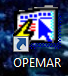
\includegraphics[scale=2]{imagen_manual_OPEMAR/OPEMAR.png}}
 \caption{Ícono del OPEMAR}
\end{center}
 \end{figure}

\newpage


\begin{itemize}
\item\textbf{PASO 2:} \\
Una vez abierto el módulo \textbf{OPEMAR}, aparecerá un la primera ventana del sistema de fondo azul, la cual deberá dirigirse a la casillas ubicadas en el emcabezado y hacer click en la casilla \textbf{CONEXIÓN}


\begin{figure} [!h]
\begin{center}
\fbox{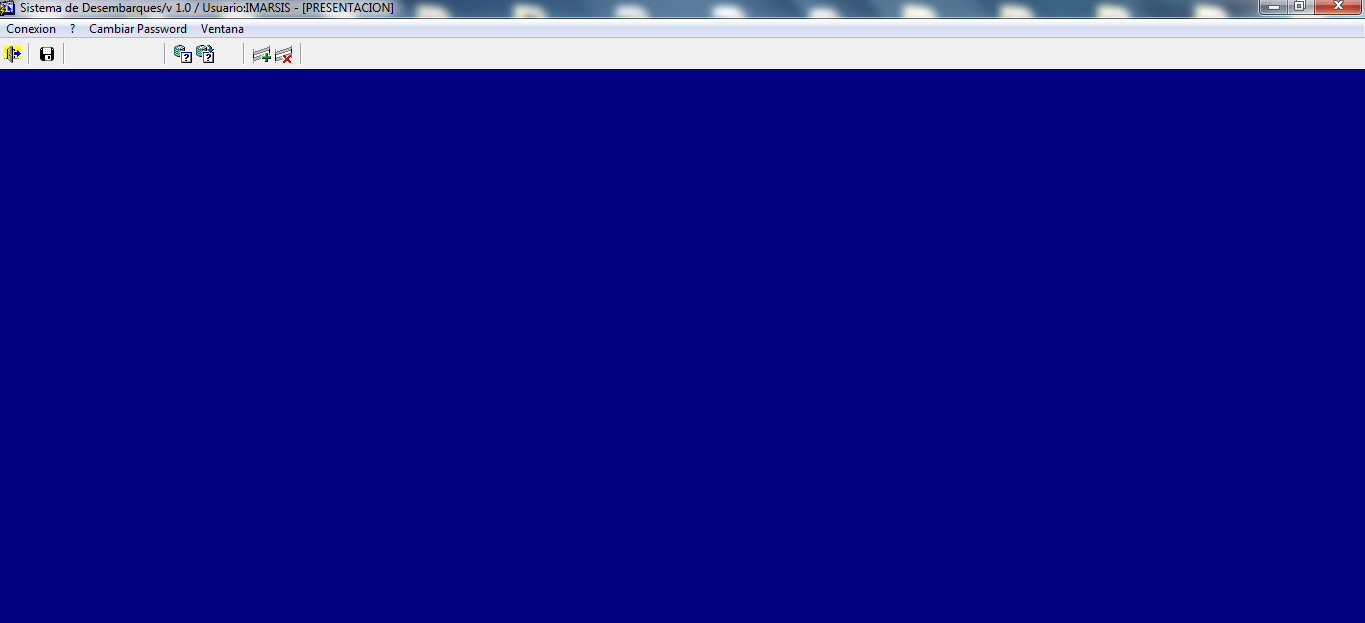
\includegraphics[scale=0.25]{imagen_manual_OPEMAR/casillafondo.png}}
 \caption{Acceso al sistema de bitácoras.}
\end{center}
 \end{figure}
 

\item\textbf{PASO 3:} \\
Luego dirigirse al emcabezado y hacer click en \textbf{Conexión}

\begin{figure} [!h]
\begin{center}
\fbox{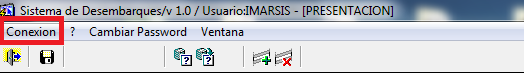
\includegraphics[scale=0.7]{imagen_manual_OPEMAR/conexion.png}}
 \caption{Acceso al sistema de bitácoras.}
\end{center}
 \end{figure}
  
\item\textbf{PASO 4:} \\
Una vez hecho clic en la casilla \textbf{conexión}, aparecerá una ventana con el acceso al sistema \textbf{OPEMAR}, solicitando los siguientes datos.\\
\subitem\textbf{Usuario:} Nombre y apellido del digitador.
\subitem\textbf{Pasword:} DNI del usuario, será visualizado en modo clave.
\end{itemize}


\begin{figure} [!h]
\begin{center}
\fbox{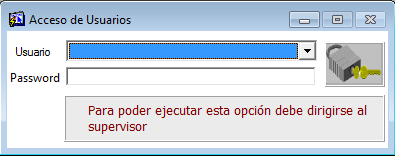
\includegraphics[scale=0.7]{imagen_manual_OPEMAR/usuario.png}}
 \caption{Acceso al sistema de bitácoras.}
\end{center}
 \end{figure}






  
  
  
\chapter { Partes de una ficha de OPEMAR en el IMARSIS}
\section{ Íconos del sistema}
\begin{itemize}
\item {Antes de insertar una ficha es necesario conocer la función de los comando del margen superior, en especial tenern en cuenta el ícono necesario para crear un nuevo registro y para salir del sistema.}
\item {Es importante que si dejará de digitar por un largo tiempo, mayor a 10 minutos, se recomienda guardar los cambios y cerrar la sesión,ya que el tener demasiado tiempo abierto programa, sin ingresar un dato, podría perder toda la información ya digitada.}
\end{itemize}


  \begin{figure} [!h]
  \begin{center}
  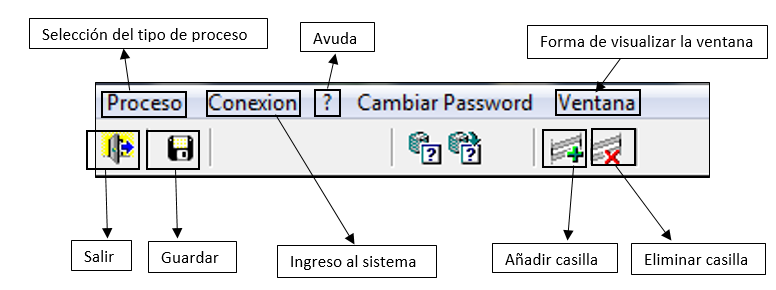
\includegraphics[scale=0.8]{imagen_manual_OPEMAR/presentacion.png}
   \caption{Íconos del encabezado.}
  \end{center}
   \end{figure}
 
 
 \newpage
 
 \begin{itemize}
 
 \item  La casilla proceso, es la casilla que deberá seleccionarse para iniciar con el proceso de ingreso de datos, esta casilla mostrará dos opciones:
  
\begin{enumerate}
 \item \textbf{Tecnología en pesca:} Esta sección permite registrar a partir de la fecha y nombre de la embarcación, el número de operación; arte de pesca, profundidad, ubicación del lance características del cardumen, capturas, pesos y mediciones. En otros términos es una de las primeras opciones que deberá seleccionarse para registrar la operación y luego de este mismo registro, posteriormente ya puede ingresar por la seccion Biología: Pelágico, toda la información biológica de la especie.
 
\item \textbf{Biología-Pelágico:} Esta sección permite el almacenamiento de la información biológica de la especie, como longitud total, peso eviscerado, sexo, madurez, longitud de gónada, peso de gónada, colecta de otolitos, que corresponde a la información extraída del muestreo biométrico de la cala. 
 \end{enumerate}
 \end{itemize}



\section{Tecnología de Pesca}

\begin{itemize}
\item Consiste en el primer registro básico y necesario para posteriormente, iniciar con el almacenamiento de la información biológica. 

 \begin{figure} [!h]
   \begin{center}
   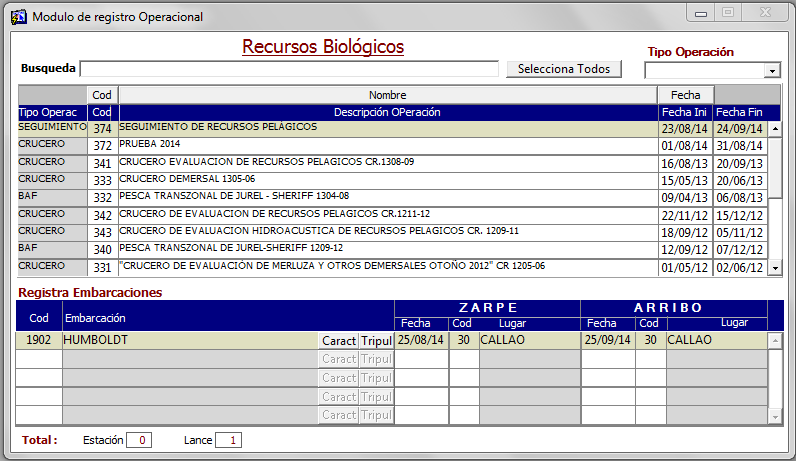
\includegraphics[scale=0.7]{imagen_manual_OPEMAR/tecno.png}
    \caption{Tecnología de pesca.}
   \end{center}
    \end{figure}
 
  \newpage
 
 \item Para familiarizarnos con la búsqueda del crucero que nos corresponde digitar o validar, debemos conocer ciertos códigos.
 
 \item Los libros empastados manejan la siguiente codificación en la pasta: \textbf{CR.0008-09  }
 
 \begin{figure} [!h]
    \begin{center}
    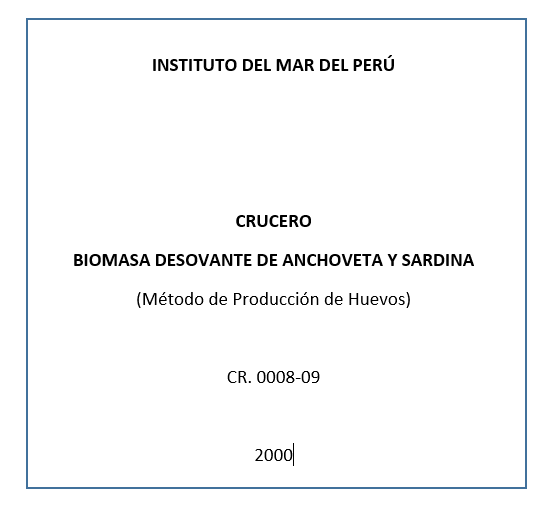
\includegraphics[scale=0.8]{imagen_manual_OPEMAR/pasta.png}
     \caption{Empastado del libro de cruceros.}
    \end{center}
     \end{figure}
 
 
 \item Para realizar la búsqueda del crucero, se deberá insertar el código: \textbf{CR-9008-09}
 \item El código se fragmenta de la siguiente manera: 
 
 
  \begin{figure} [!h]
     \begin{center}
     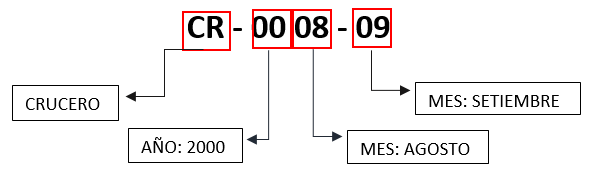
\includegraphics[scale=0.8]{imagen_manual_OPEMAR/CODIGO.png}
      \caption{Empastado del libro de cruceros.}
     \end{center}
      \end{figure}
 
 \item De manera que el código se deberá colocar en el buscador de la casilla: \textbf{TECNOLOGÍA DE PESCA.}
 
 
 \begin{figure} [!h]
      \begin{center}
      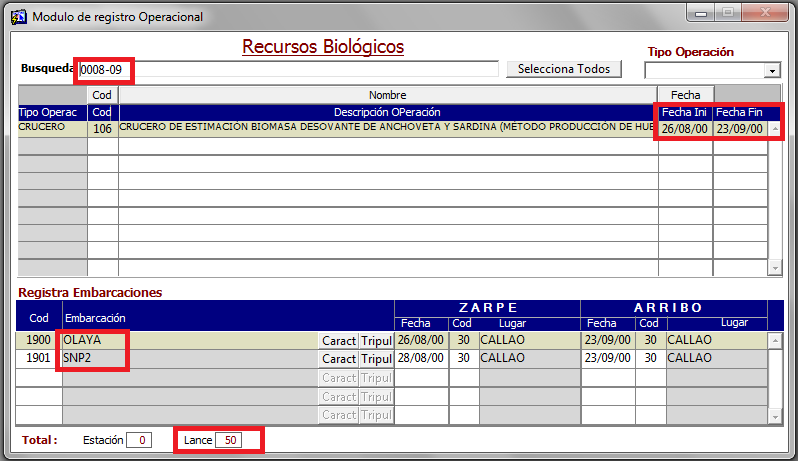
\includegraphics[scale=0.7]{imagen_manual_OPEMAR/casilla1.png}
       \caption{Empastado del libro de cruceros.}
      \end{center}
       \end{figure}
 
 \item Considerar la siguiente información: 
 \begin{enumerate}

\item  \textbf{Búsqueda :} Casilla donde colocar el código.
\item \textbf{Fecha Inicio - Final:} Duración del crucero
\item \textbf{Embarcación:} Dentro de este crucero, se almacena la información de dos embarcaciones que recogieron información durante la temporada de agosto y setiembre.
\item  \textbf{Lance:} La cantidad de lances por embarcación Olaya y si se desea ver la cantidad de lances para la embarcación SNP2, hacer click en el respectivo reglón.
\end{enumerate}

\item Hacer click en la casilla \textbf{COD} de la embarcación.
 
  \begin{figure} [!h]
       \begin{center}
      \fbox{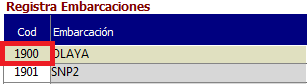
\includegraphics[scale=0.81]{imagen_manual_OPEMAR/casilla2.png}}
        \caption{Empastado del libro de cruceros.}
       \end{center}
        \end{figure}
  \end{itemize}
 
 
 \newpage


 \subsection{ Partes de la casilla Tecnología de Pesca}
 \begin{itemize}
\item [] Una vez hecho click en la casilla \textbf{COD=Código}, correspondiente a la embarcación, aparecerá el siguiente recuadro. Sectores de la casilla: \textbf{BITÁCORA}
 \end{itemize}
 
         \begin{figure} [!h]
                 \begin{center}
               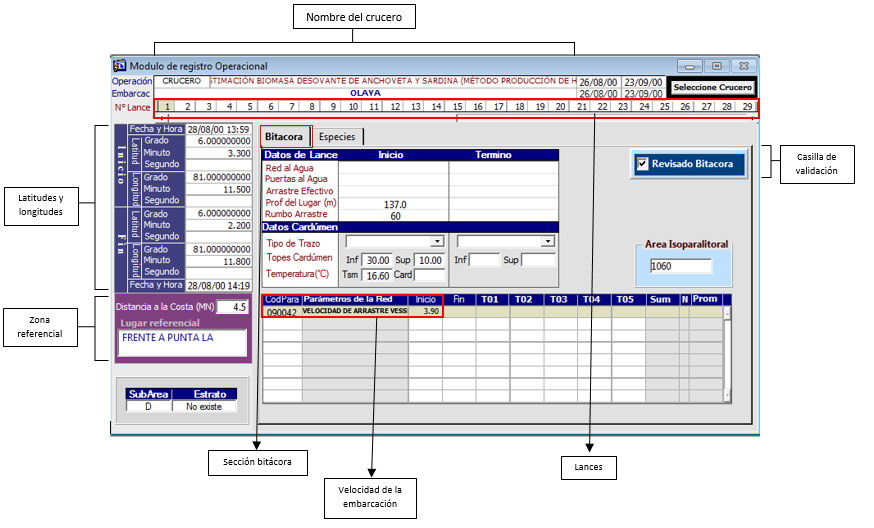
\includegraphics[scale=0.6]{imagen_manual_OPEMAR/casilla4.png}
                  \caption{Tecnología de Pesca: Bitácora.}
                 \end{center}
                  \end{figure}
      
      
 
 \begin{enumerate}
 \item Operación = Nombre del crucero.
 \item Embarcación= Olaya 
 \item Número de lance=
 \item Datos del lance= 
 \begin{enumerate}
\item Red al agua 
\item Puertas al agua 
\item Arrastre efectivo
\item Profundidad del lugar(m)
\item Rumbo arrastre
\item Datos Cardúmen 
\end{enumerate}
\end{enumerate}
\newpage
\begin{itemize}
\item Sectores de la casilla: \textbf{ESPECIES}

        
 \begin{figure} [!h]
 \begin{center}
 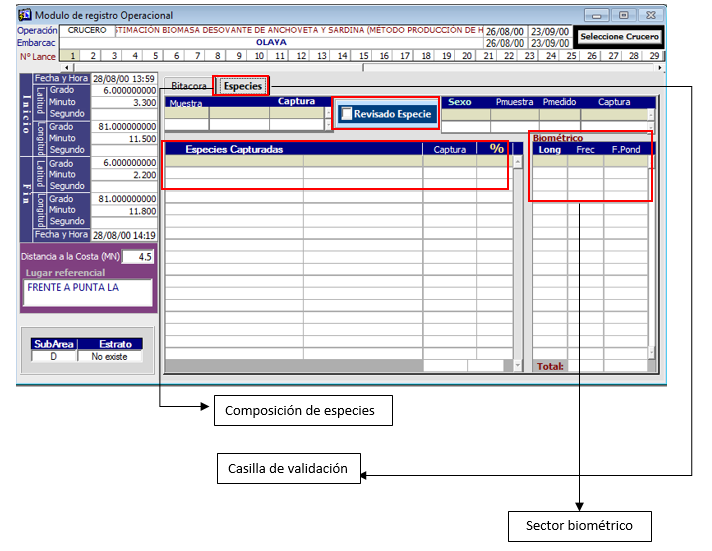
\includegraphics[scale=0.52]{imagen_manual_OPEMAR/casilla5.png}
    \caption{Tecnología de Pesca: Bitácora.}
  \end{center}
\end{figure}





\begin{enumerate}
\item Muestra
\item Captura
\item Especies capturadas
\item Captura
\item Biométrico 
\begin{enumerate}
\item Longitud
\item Frecuencia
\item Frecuencia Ponderada
\end{enumerate}
\end{enumerate}
 \end{itemize} 

\newpage
 \section{Partes de la casilla Biología - Pelágico}
 
 \begin{itemize}
 \item [] Para ingresar a la sección \textbf{BIOLOGÍA-PELÁGICO}, es necesario cerrar la sesión en TECNOLOGÍA DE PESCA, de la siguiente forma, a través del ícono: \textbf{SALIR }
 
         
         
\begin{figure} [!h]
\begin{center}
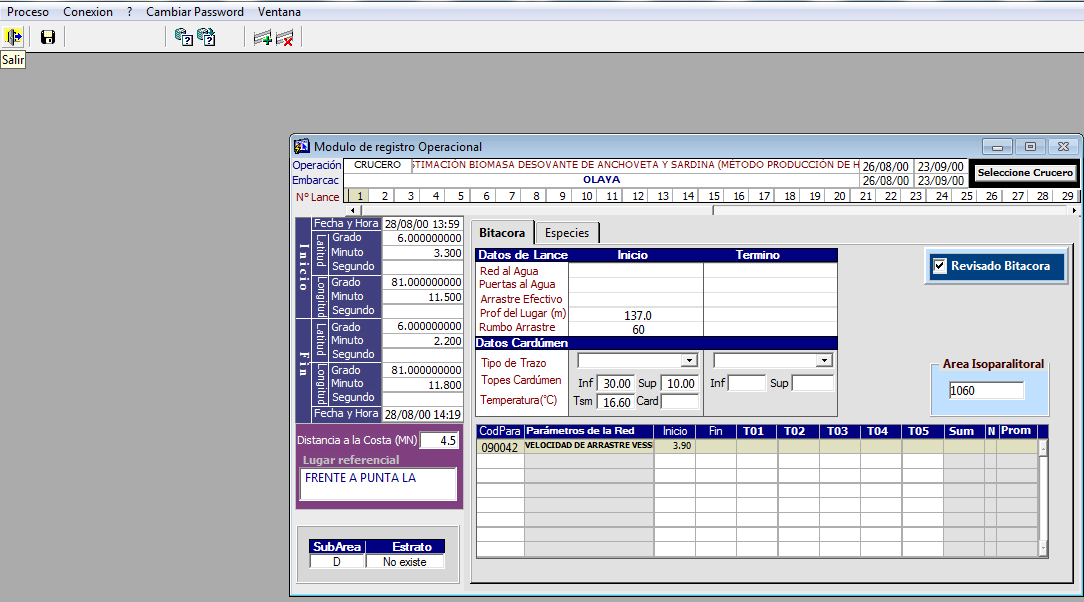
\includegraphics[scale=0.35]{imagen_manual_OPEMAR/salir.png}
\caption{Tecnología de Pesca: Bitácora.}
\end{center}
\end{figure}
         
\item Luego se deberá seleccionar las casillas en el siguiente orden: 
\item [] Operaciones en el mar: BIOLOGÍA: PELÁGICO, hay que considerar que por esta seccion solo se podrá hacer ingreso de información biológica, por lo que no se podrá modificar ningún dato de la casilla de tecnología.

\begin{figure} [!h]
\begin{center}
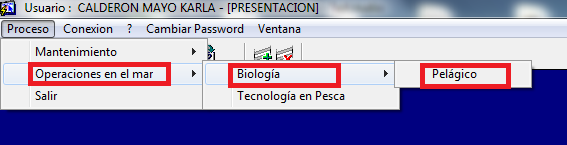
\includegraphics[scale=0.4]{imagen_manual_OPEMAR/rojo.png}
\caption{Tecnología de Pesca: Bitácora.}
\end{center}
\end{figure}

\item Luego figurará la siguiente casilla

\begin{figure} [!h]
\begin{center}
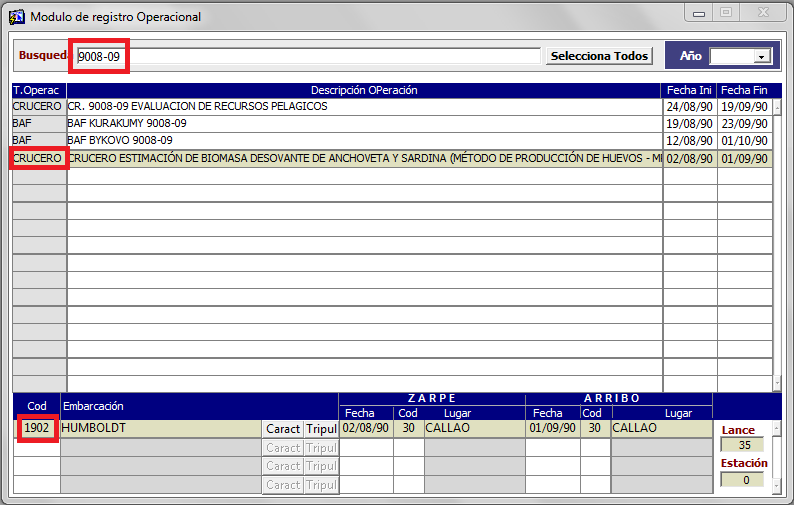
\includegraphics[scale=0.30]{imagen_manual_OPEMAR/rojo1.png}
\caption{Búsqueda por Biología: Pelágico.}
\end{center}
\end{figure}


\item Dentro de la casilla Biología- Pelágico, se podrá visualizar todos los módulos internos, que solo podrán ser modificados e eliminados a traves de TECNOLOGÍA DE PESCA, queda claro que solo el módulo Biología-Pelágico, servirá para añadir la información biológica de la captura ya ingresa  por tecnología. 


\begin{figure} [!h]
\begin{center}
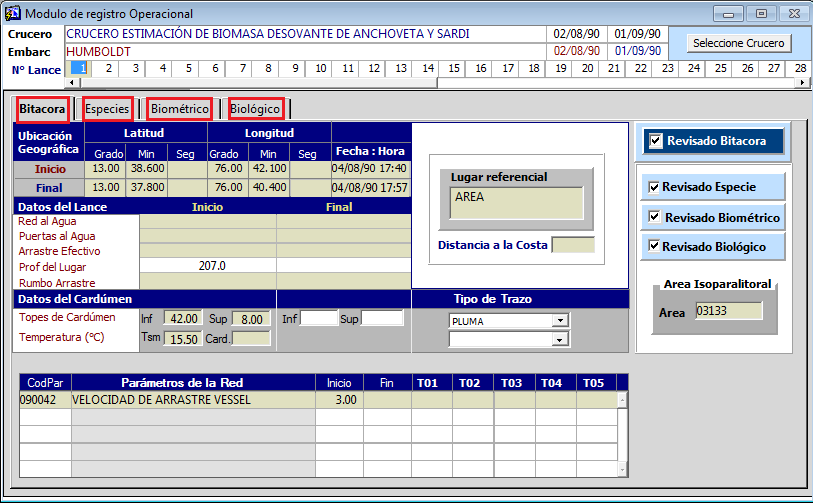
\includegraphics[scale=0.35]{imagen_manual_OPEMAR/casillasardina.png}
\caption{Búsqueda por Biología: Pelágico.}
\end{center}
\end{figure}

\begin{enumerate}
\item\textbf{ Bitácora:} Toda la información visualizada en este sector fue añadida a través de Tecnología de Pesca, por lo cual cambio no podrá ser añadido e eliminado.

\begin{figure} [!h]
\begin{center}
\fbox{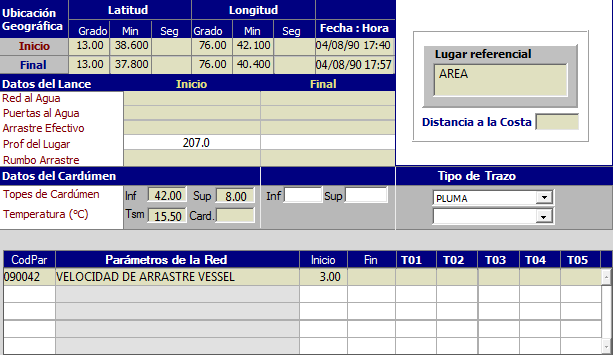
\includegraphics[scale=0.35]{imagen_manual_OPEMAR/bita.png}}
\caption{Búsqueda por Biología: Pelágico.}
\end{center}
\end{figure}


\item \textbf{Especies:} De la misma forma toda la información mostrada fue ingresada por Tecnología de Pesca.
   
\begin{figure} [!h]
\begin{center}
\fbox{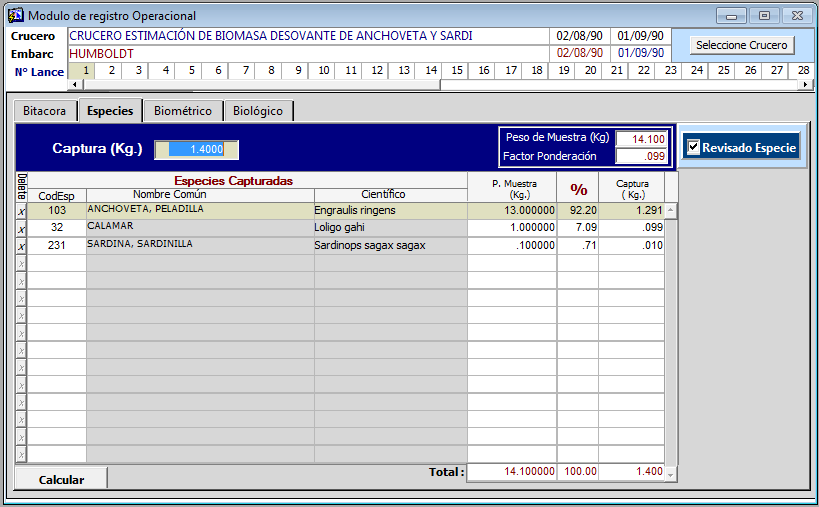
\includegraphics[scale=0.3]{imagen_manual_OPEMAR/cor.png}}
\caption{Búsqueda por Biología: Pelágico.}
\end{center}
\end{figure}

   
\newpage


\item \textbf{Biométrico:} De la misma manera esta sección fue ingresada por Tecnología de Pesca.

\begin{figure} [!h]
\begin{center}
\fbox{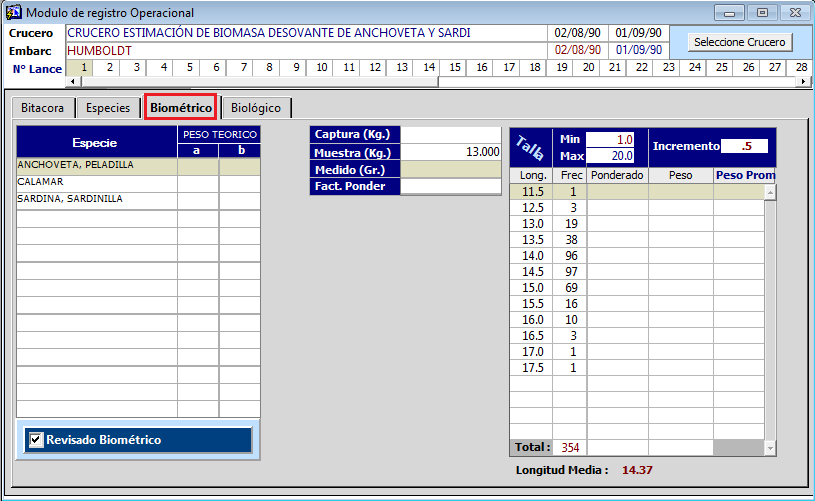
\includegraphics[scale=0.3]{imagen_manual_OPEMAR/biome.png}}
\caption{Sección: Biométrico.}
\end{center}
\end{figure}


\item \textbf{Biológico:}  Solo se podrá añadir información biológica de las especies que se ingresaron a travé de la casilla Tecnología de Pesca.

\begin{figure} [!h]
\begin{center}
\fbox{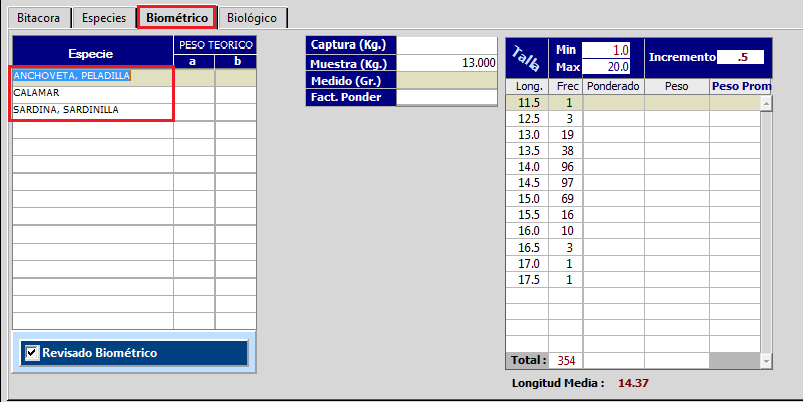
\includegraphics[scale=0.4]{imagen_manual_OPEMAR/biome1.png}}
\caption{Sección: Biométrico.}
\end{center}
\end{figure}

\item [] En la sección biológica, figurarán solo las especies que se encuentran añadidas en el biométrico. 


\begin{figure} [!h]
\begin{center}
\fbox{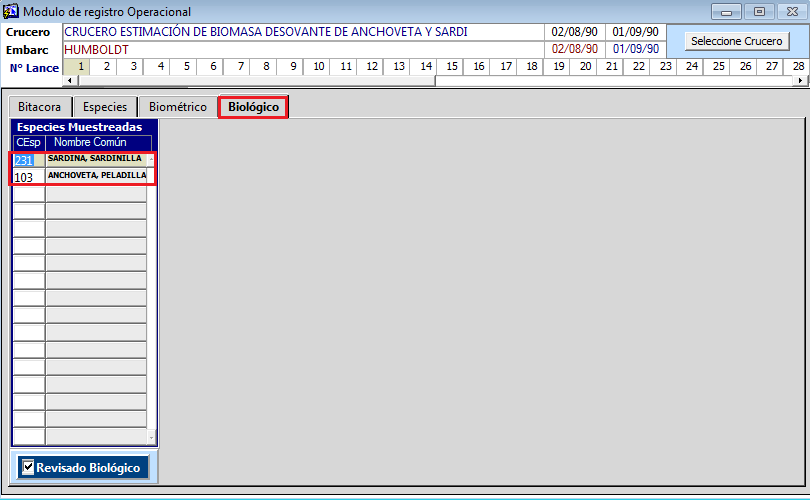
\includegraphics[scale=0.38]{imagen_manual_OPEMAR/biome2.png}}
\caption{Sección: Biométrico.}
\end{center}
\end{figure}

\item [] Para añadir la información biológica de la especie, deberá hacerse click en el cuadro de la especie y consecuentemente figurará

\begin{figure} [!h]
\begin{center}
\fbox{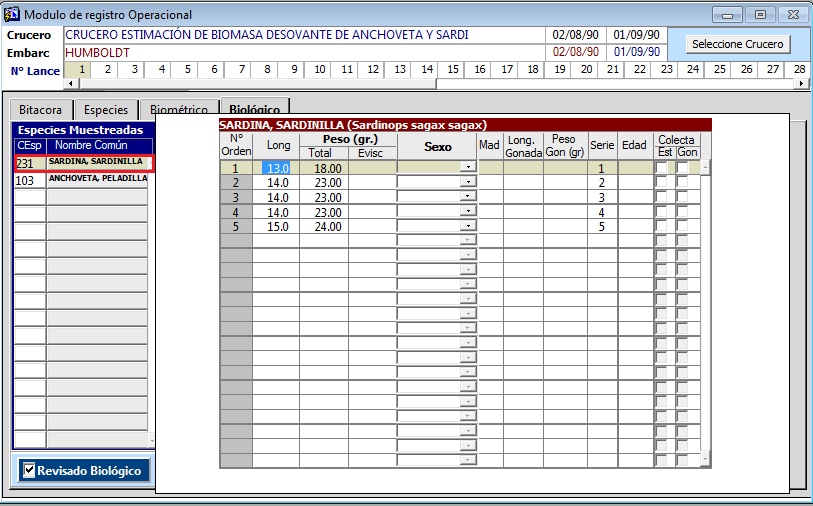
\includegraphics[scale=0.38]{imagen_manual_OPEMAR/biome5.png}}
\caption{Sección: Biométrico.}
\end{center}
\end{figure}

\end{enumerate}


\subsection{Casilla biológica:} 
\begin{itemize}
\item [] La casilla biológica, solicitará los siguientes datos. 
\end{itemize}

\begin{figure} [!h]
\begin{center}
\fbox{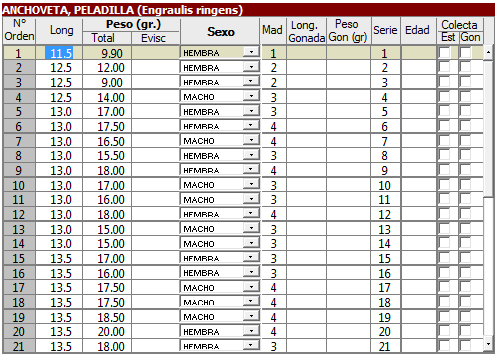
\includegraphics[scale=0.8]{imagen_manual_OPEMAR/casillabio.png}}
\caption{Sección: Biométrico.}
\end{center}
\end{figure}


\begin{enumerate}
\item \textbf{Número de orden:} Orden consecutivo en el que se ingresan los datos.
\item \textbf{Longitud(cm):} Casilla que contiene el rango de talla. 
\item \textbf{Peso (gr):} Peso del pez, expresado en gramos 
\begin{enumerate}
\item \textbf{Total(gr):} Peso del pez completo, sin eviscerar.
\item \textbf{Eviscerado:} Peso del pez, sin estómago, hígado y gónada.
\end{enumerate}
\item \textbf{Sexo:} Define el sexo del especimen.
\begin{enumerate}
 \item\textbf{{Ambos sexos:}} En el caso de la que la ficha lo indique.
 \item{\textbf{Hembra:}} Si el sexo del especimen es hembra, esta información se ingresará como el número: \textbf{0}
 \item \textbf{Indeterminado}: En el caso de no poder haber sido definido, ya sea por el estadío juvenil.
 \item \textbf{Macho}: Si el sexo del especimen es macho, esta información se ingresará como el número\textbf{1}
 \item \textbf{Sin dato:} En el caso de no figurar la información en ficha, colocar sin dato.
 \end{enumerate}


\begin{figure} [!h]
\begin{center}
\fbox{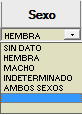
\includegraphics[scale=1.2]{imagen_manual_OPEMAR/sexo.png}}\caption{Selección: Sexo.}
\end{center}
\end{figure}


\item \textbf{Madurez:} Información que permite saber si la especie logró alcanzar la capacidad para reproducirse, para la cual se define con un sistema de escalas a través de un análisis en gónadas cuya determinación depende del grosor, consistencia y color. Las escalas son ingresadas en números ordinales. Por ejemplo: 1 - 2 - 3 ...7.

\begin{figure} [!h]
\begin{center}
\fbox{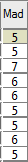
\includegraphics[scale=1.2]{imagen_manual_OPEMAR/madu.png}}\caption{Selección: Sexo.}
\end{center}
\end{figure}



\item \textbf{Longitud de gónada: } Las longitudes en gónadas son ingresadas en milímetros (mm) y es posible que en las fichas la longitud haya sido registrada en (cm), para lo cual esto datos al ser ingresados al sistema, estas deben convertirse a (mm).
 
 
\item \textbf{Peso de gónada:} Corresponde el peso de los testículos y los sacos ováricos, ingresados en gramos(g).


\item \textbf{Serie:} Secuencia de la colecta de otolitos.
\item \textbf{Edad:} Determinada, por la lectura de otolitos.
\item \textbf{Colecta:} No necesariamente obligatoria.
\begin{enumerate}
\item \textbf{Estómago:} Marcar con un check en el caso de figurar colecta de estómago en la ficha.

\begin{figure} [!h]
\begin{center}
\fbox{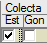
\includegraphics[scale=1.2]{imagen_manual_OPEMAR/estomago.png}}\caption{Colecta: Estómago}
\end{center}
\end{figure}

\item \textbf {Gónada:} Marcar con un check  en el caso de figurar la colecta de gónadas. 
\end{enumerate}
\end{enumerate}


\begin{figure} [!h]
\begin{center}
\fbox{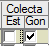
\includegraphics[scale=1.2]{imagen_manual_OPEMAR/gonada.png}}\caption{Colecta: Gónada}
\end{center}
\end{figure}

\end{itemize}
 
\chapter {Partes de la ficha: Formulario de Muestreo Capturas a Bordo}
 
\begin{itemize}
\item  En esta capítulo, el objetivo es conocer los sectores y partes de una ficha perteneciente a Muestreo Capturas a Bordo, dichas fichas son las entregadas y agrupadas por temporadas y viajes, que finalmente son entregadas para digitar.
\end{itemize}

 
 \begin{figure} [!h]
 \begin{center}
 \fbox{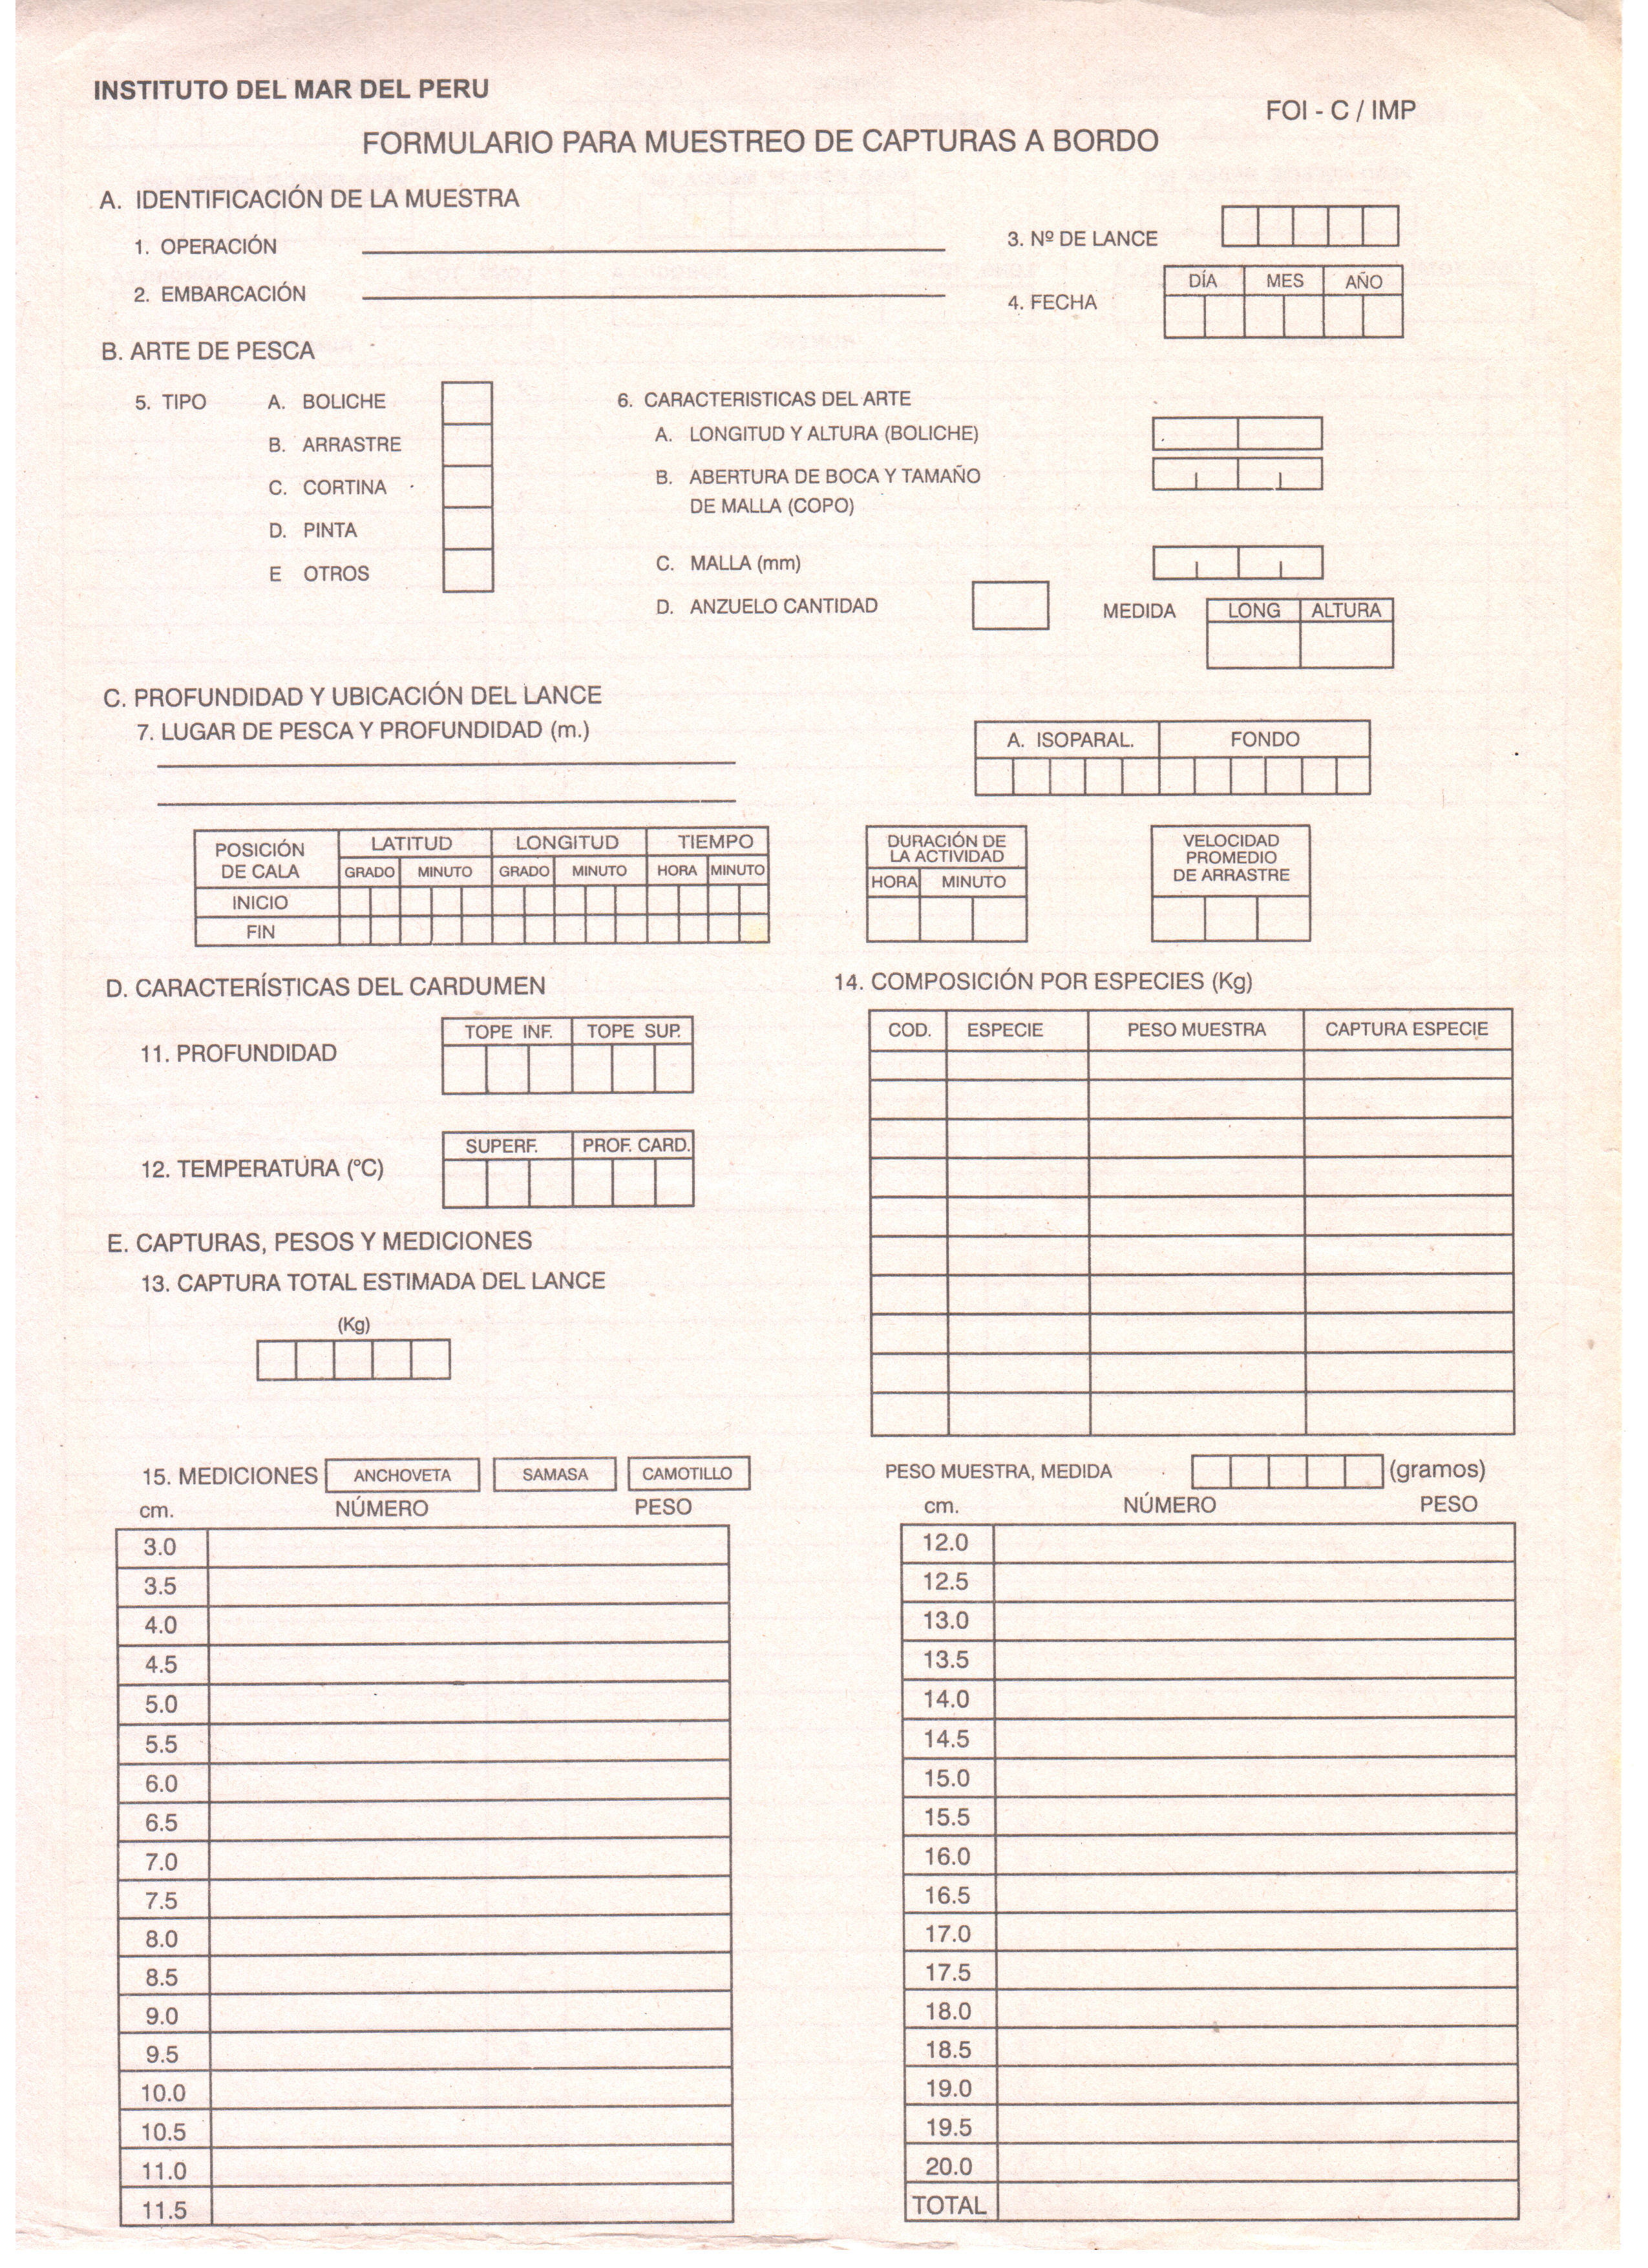
\includegraphics[scale=0.38]{imagen_manual_OPEMAR/ficha.jpg}}\caption{Ficha: Formulario de Muestreo Capturas a Bordo}
 \end{center}
 \end{figure}
 
  \section{Identificación de la muestra}
  
   \begin{figure} [!h]
    \begin{center}
    \fbox{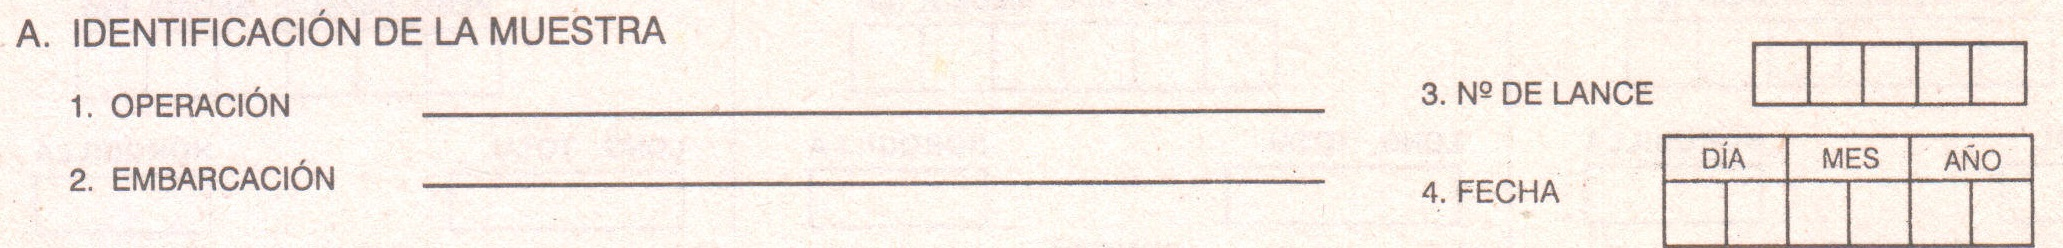
\includegraphics[scale=0.7]{imagen_manual_OPEMAR/secciona.jpg}} %\caption{Ficha: Secci�n A: Indentificaci�n de la muestra}
    \end{center}
    \end{figure}
  
  \begin{itemize}
  \item La sección A: Está referida a la información general de la operación, embarcación, Número de lance y fecha.
 \end{itemize}
 
 \begin{enumerate}
 \item\textbf{ Operación:} El tipo de operación está orientado al objetivo de estudio del crucero. Ejemplo: 
 \item [] Crucero Biomasa Desovante de Anchoveta y Sardina.
 \item[] Crucero de Evaluación de Recursos Pelágicos.
 \item \textbf{Embarcación:} Son las embarcaciones utilizadas para realizar el estudio, como : El  Imarpe IV, Imarpe V, B.I.C José Olaya Balandra, Humboldt.
 
 \item\textbf{Número de lance:} Número de calas, realizadas dentro de la operación.
 \item \textbf{Fecha:} Fecha de inicio y final de la operación.

\end{enumerate} 
 



\section{Artes de Pesca}

\begin{figure} [!h]
  \begin{center}
  \fbox{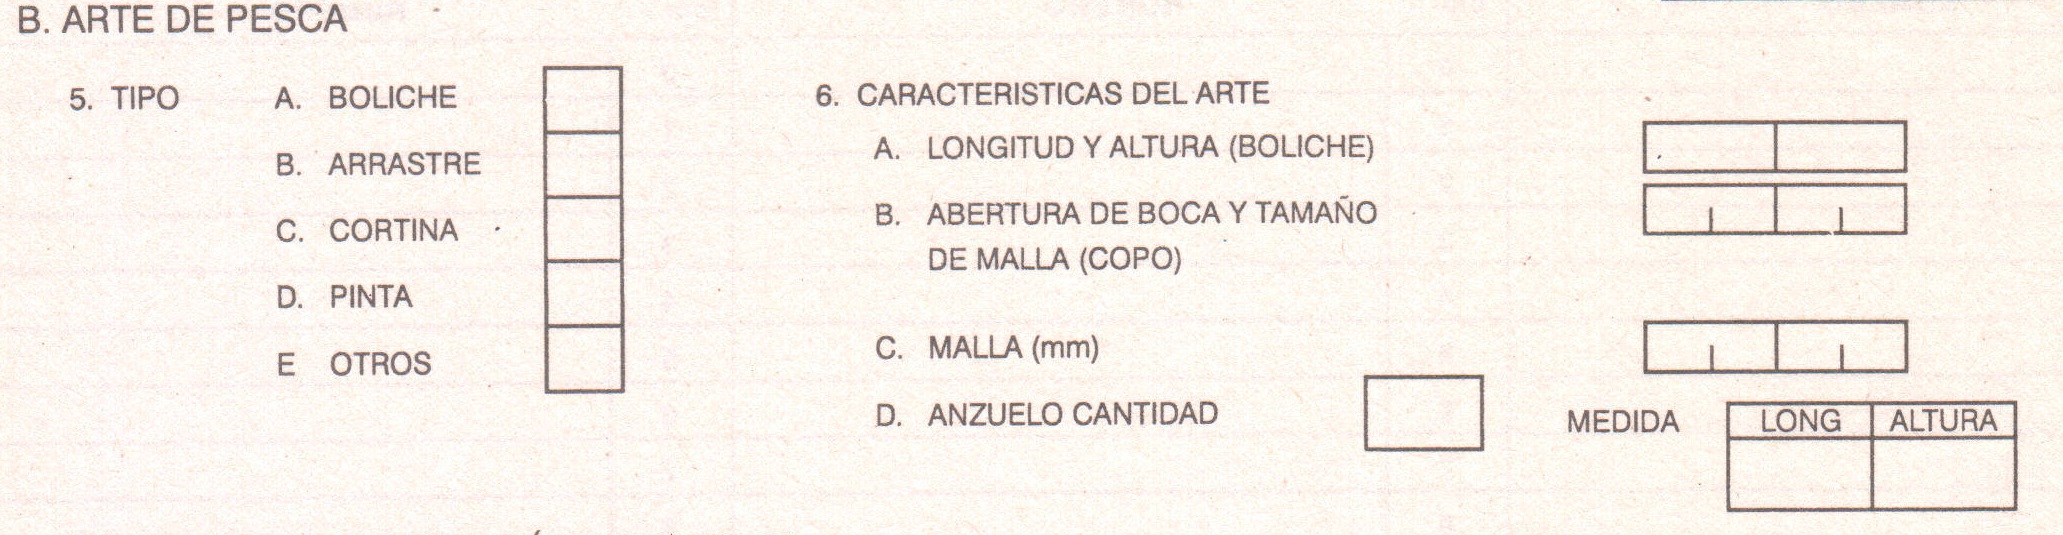
\includegraphics[scale=0.7]{imagen_manual_OPEMAR/b.jpg}} %\caption{Ficha: Secci�n A: Indentificaci�n de la muestra}
  \end{center}
  \end{figure}

\begin{enumerate}
\item Tipos de arte de pesca
\begin{enumerate}
\item \textbf{Boliche:} Red que en uno de sus extremos tiene muchos plomos y en el otro varios corchos, para impedir que toda ella se sumerja en el agua. Tírase de ambos con botes o desde tierra.
\item \textbf{Arrastre:} Son aquellas que mediante uno o dos cables de tracción, con o sin puertas, arrastran, por el fondo o entre aguas una red, de aspecto similar a un embudo, con objeto de capturar a los organismos que allá habitan.
\item \textbf{Cortina:} Una red cortina apresa los peces por las agallas (branquias) y funciona como sigue: el hilo de los paños es muy delgado y los peces o no lo ven, o la red está calada de manera que los atrapa. Las mallas de la red están completamente abiertas. 

\item \textbf{Pinta:} Son artes de línea en mano, compuesta de anzuelos y muchas veces acompañada de carnadas.
\item \textbf{Otros:} Artes como cortina agallera, cortina transmallo, entre otros.
\end{enumerate}
\item Características del arte
\begin{itemize}
\item Longitud y altura (Boliche): largo y ancho de la red.
\item Abertura de boca y tamaño de la malla (COPO):Se denomina COPO, al bolso a manera de saco que recoge la captura contenida en red.
\item Malla (mm): Calibre y grosor de la red.
\item Anzuelo : Cantidad y Número de anzuelos empleados.
\end{itemize}
\end{enumerate}

\section{Profundidad y ubicación del lance}


 \begin{figure} [!h]
  \begin{center}
   \fbox{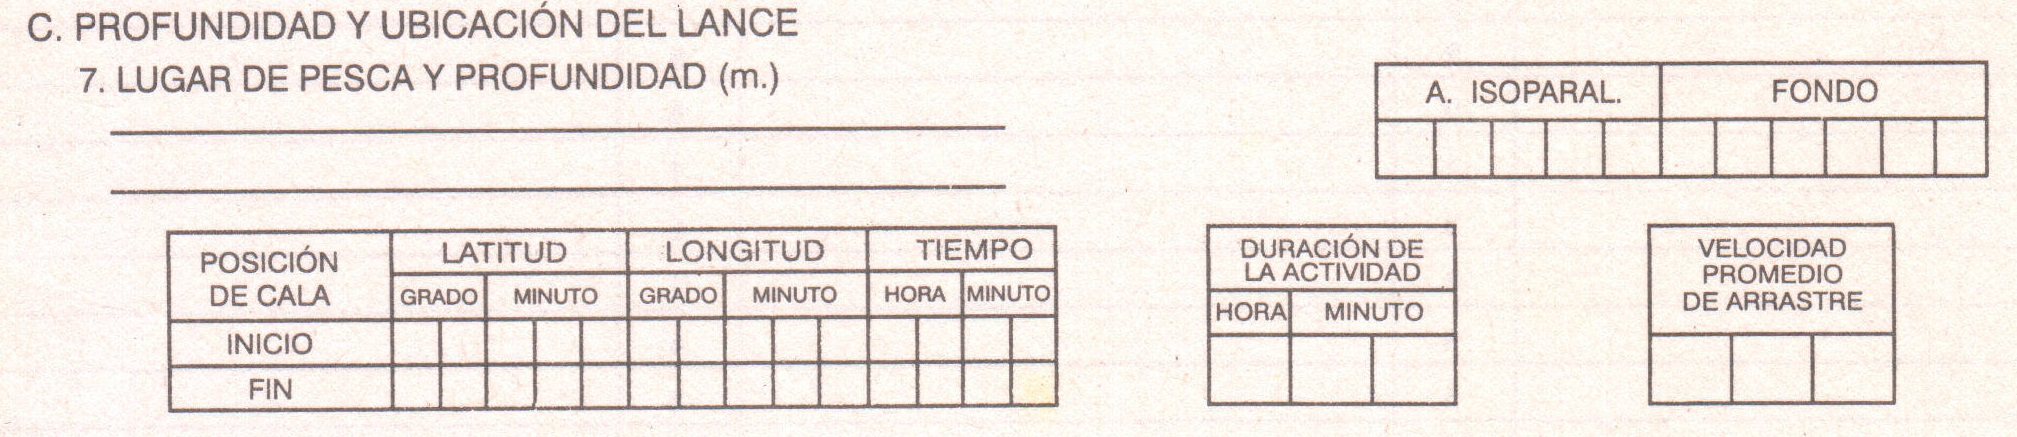
\includegraphics[scale=0.7]{imagen_manual_OPEMAR/c.jpg}} %\caption{Ficha: Secci�n A: Indentificaci�n de la muestra}
   \end{center}
   \end{figure}
  
\begin{enumerate}

\item \textbf{Lugar de pesca y profundidad (m):} El lugar de pesca también es conocido como lugar de referencia.
\item Posición de la cala: La posición se encuentra basada por las coordenadas (latitud y longitud).
\item Area Isoparalitoral: Expresa por 4 códigos que indican...

% % % % % % % ver explicaci�n. % % % % % % % % % %
\item Fondo
\item Duración de la actividad 
\item Velocidad promedio de arrastre
\end{enumerate}


\section{Características del cardúmen}

 \begin{figure} [!h]
  \begin{center}
   \fbox{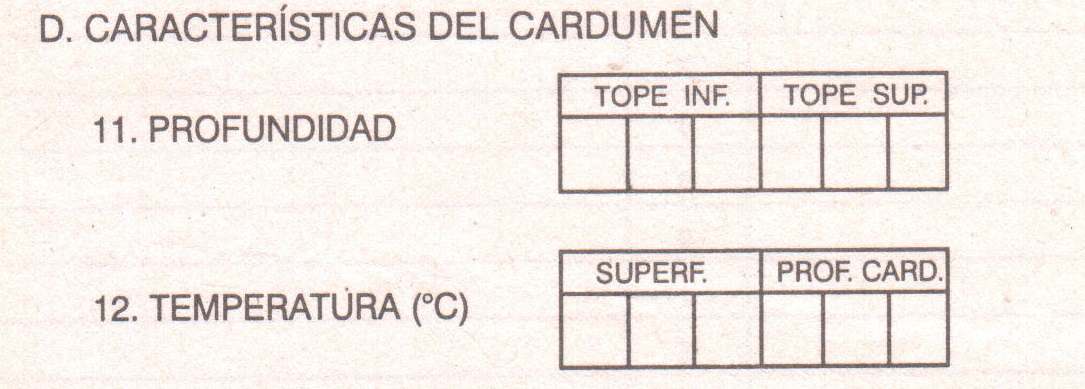
\includegraphics[scale=0.7]{imagen_manual_OPEMAR/d.jpg}} %\caption{Ficha: Secci�n A: Indentificaci�n de la muestra}
   \end{center}
   \end{figure}

\begin{enumerate}
\item Profundidad
\item Temperatura
\end{enumerate}



\section{Capturas, pesos y mediciones}


\begin{figure} [!h]
  \begin{center}
   \fbox{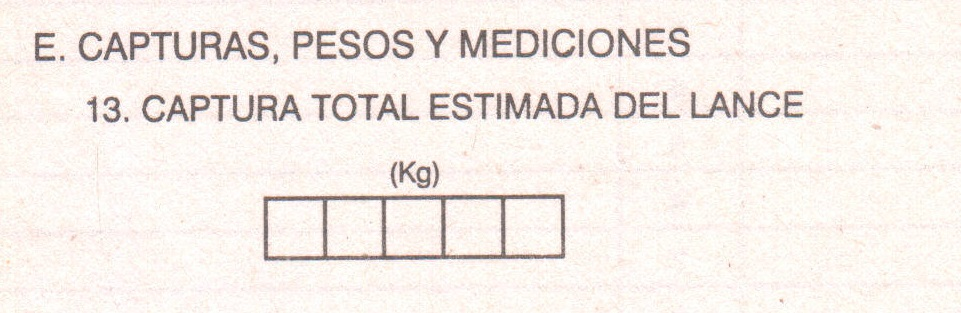
\includegraphics[scale=0.7]{imagen_manual_OPEMAR/e.jpg}} %\caption{Ficha: Secci�n A: Indentificaci�n de la muestra}
   \end{center}
   \end{figure}

\begin{enumerate}
\item Composición por especies (Kg)
\begin{enumerate}
\item Cod:
\item Especie
\item Peso muestra
\item Captura especie
\end{enumerate}
\end{enumerate}


\begin{figure} [!h]
  \begin{center}
   \fbox{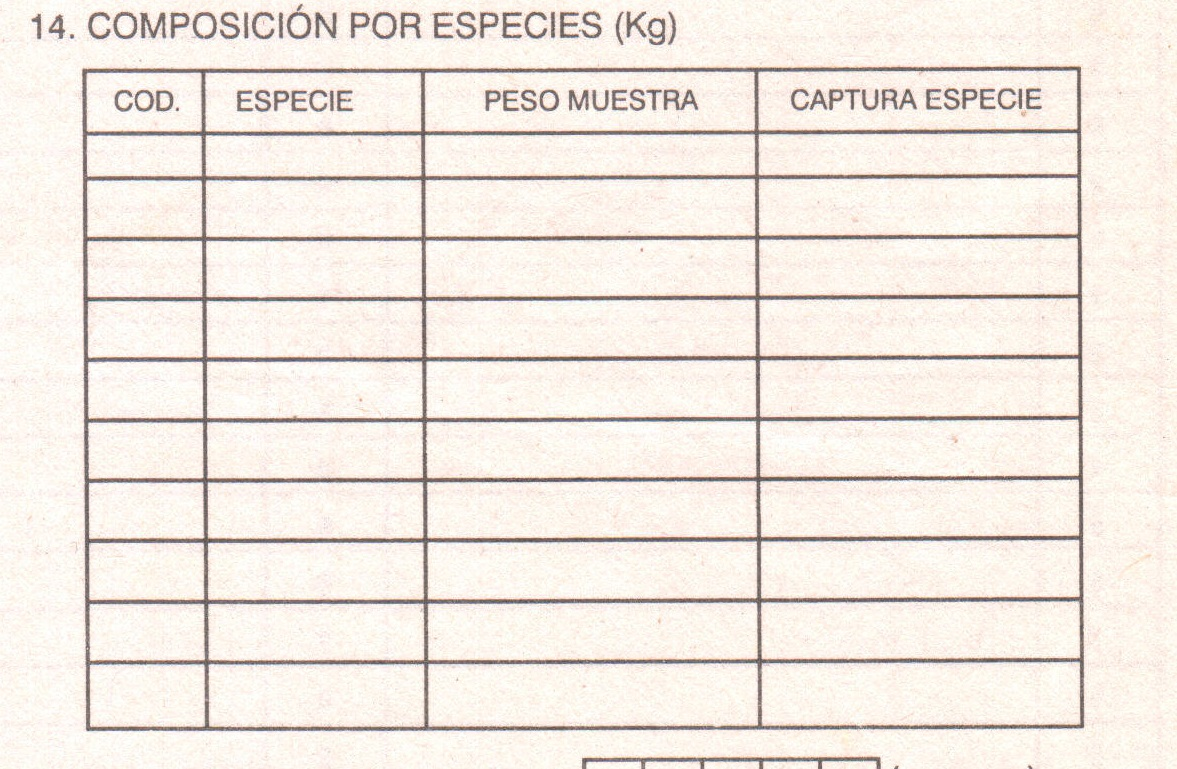
\includegraphics[scale=0.7]{imagen_manual_OPEMAR/f.jpg}} %\caption{Ficha: Secci�n A: Indentificaci�n de la muestra}
   \end{center}
   \end{figure}


\section{Mediciones}

\begin{figure} [!h]
  \begin{center}
   \fbox{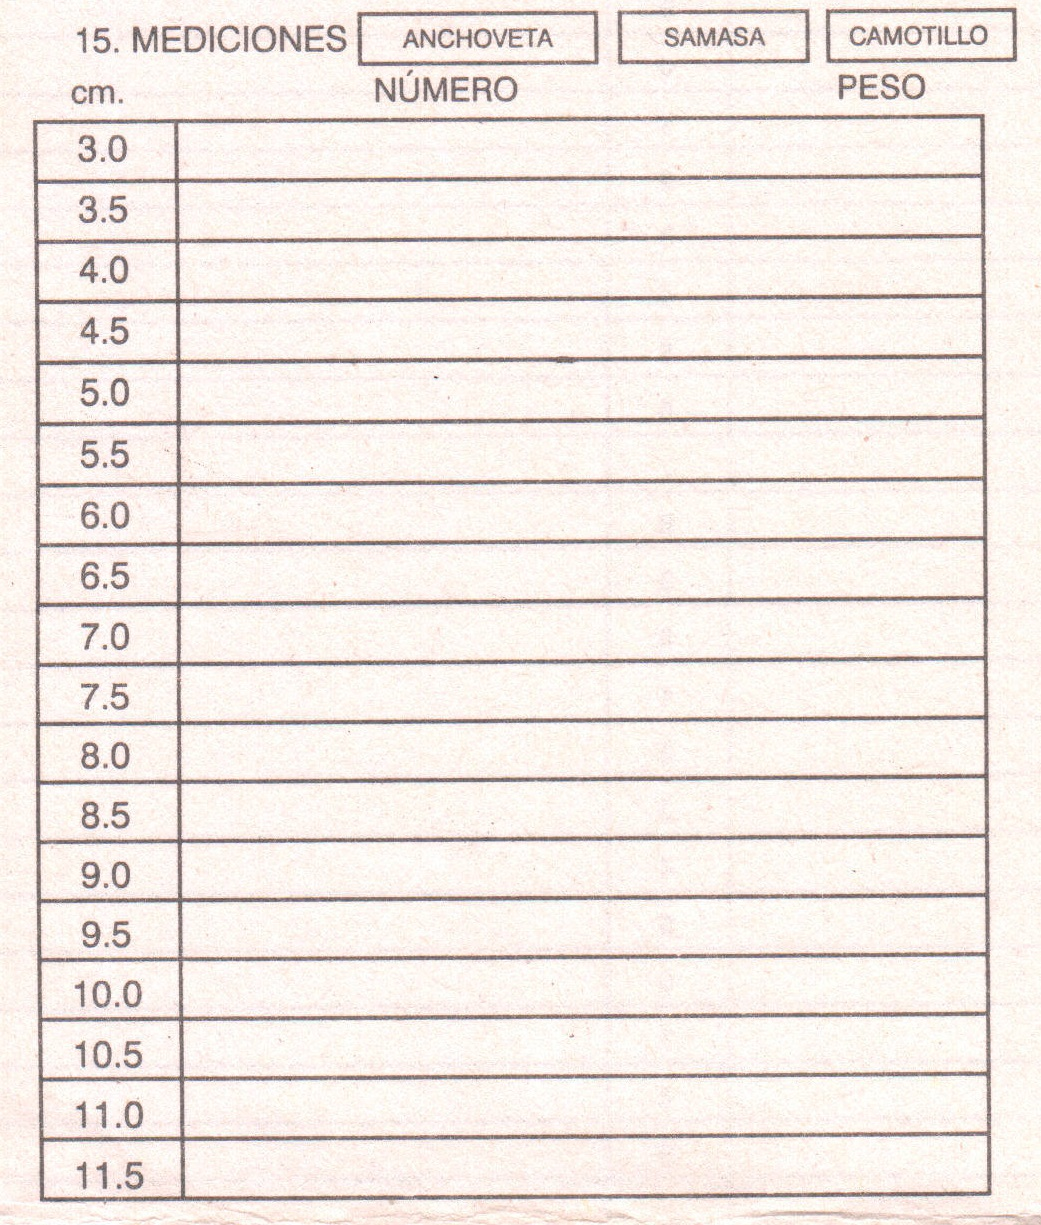
\includegraphics[scale=0.6]{imagen_manual_OPEMAR/ficha12.jpg}} %\caption{Ficha: Secci�n A: Indentificaci�n de la muestra}
   \end{center}
   \end{figure}

\section{Peso muestra, medida (gr)}

\begin{figure} [!h]
  \begin{center}
   \fbox{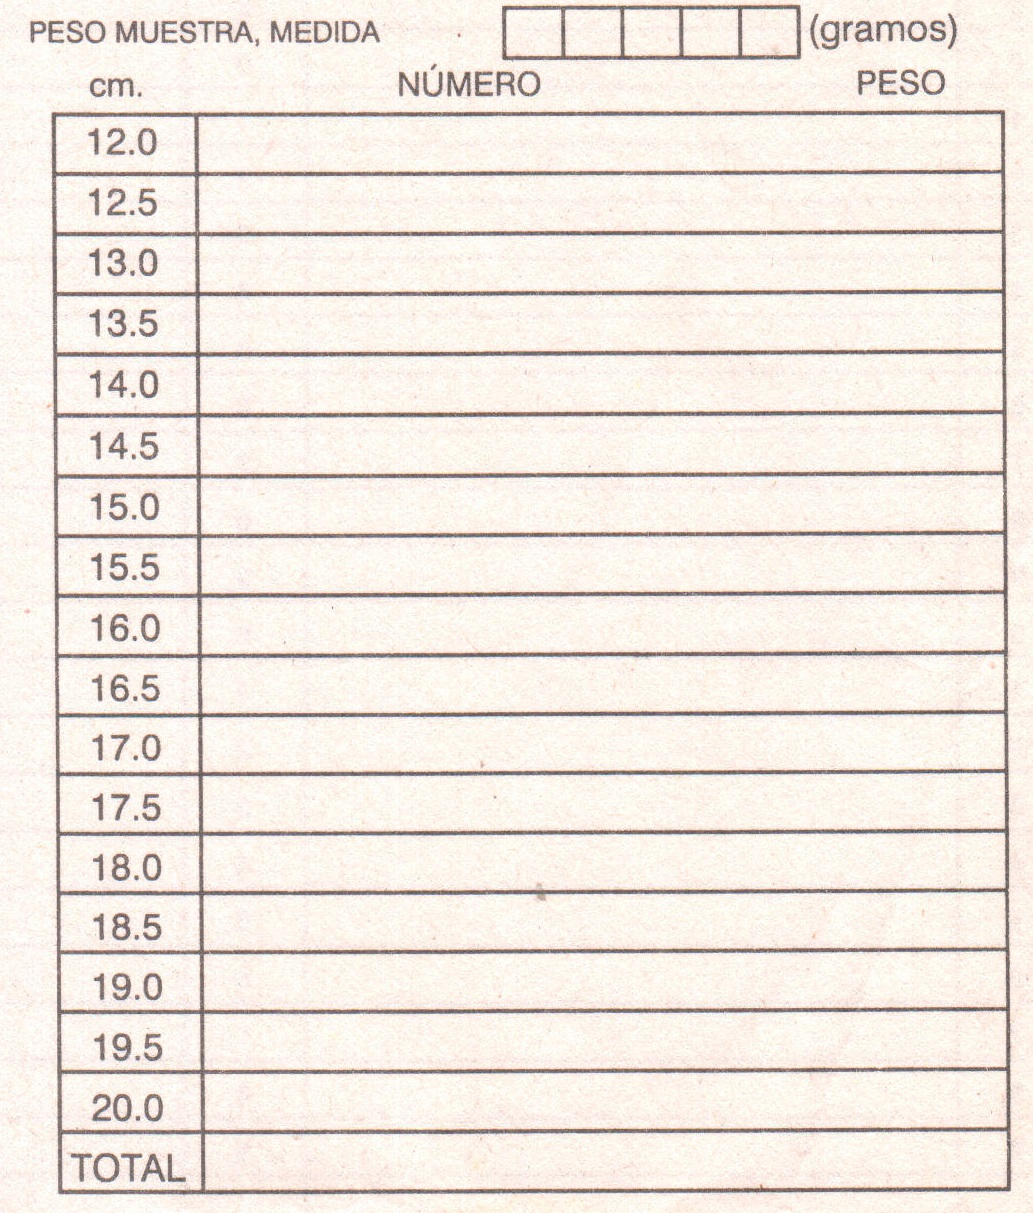
\includegraphics[scale=0.6]{imagen_manual_OPEMAR/ficha78.jpg}} %\caption{Ficha: Secci�n A: Indentificaci�n de la muestra}
   \end{center}
   \end{figure}
 
 \section{Para otras especies}
 
 \begin{figure} [!h]
   \begin{center}
    \fbox{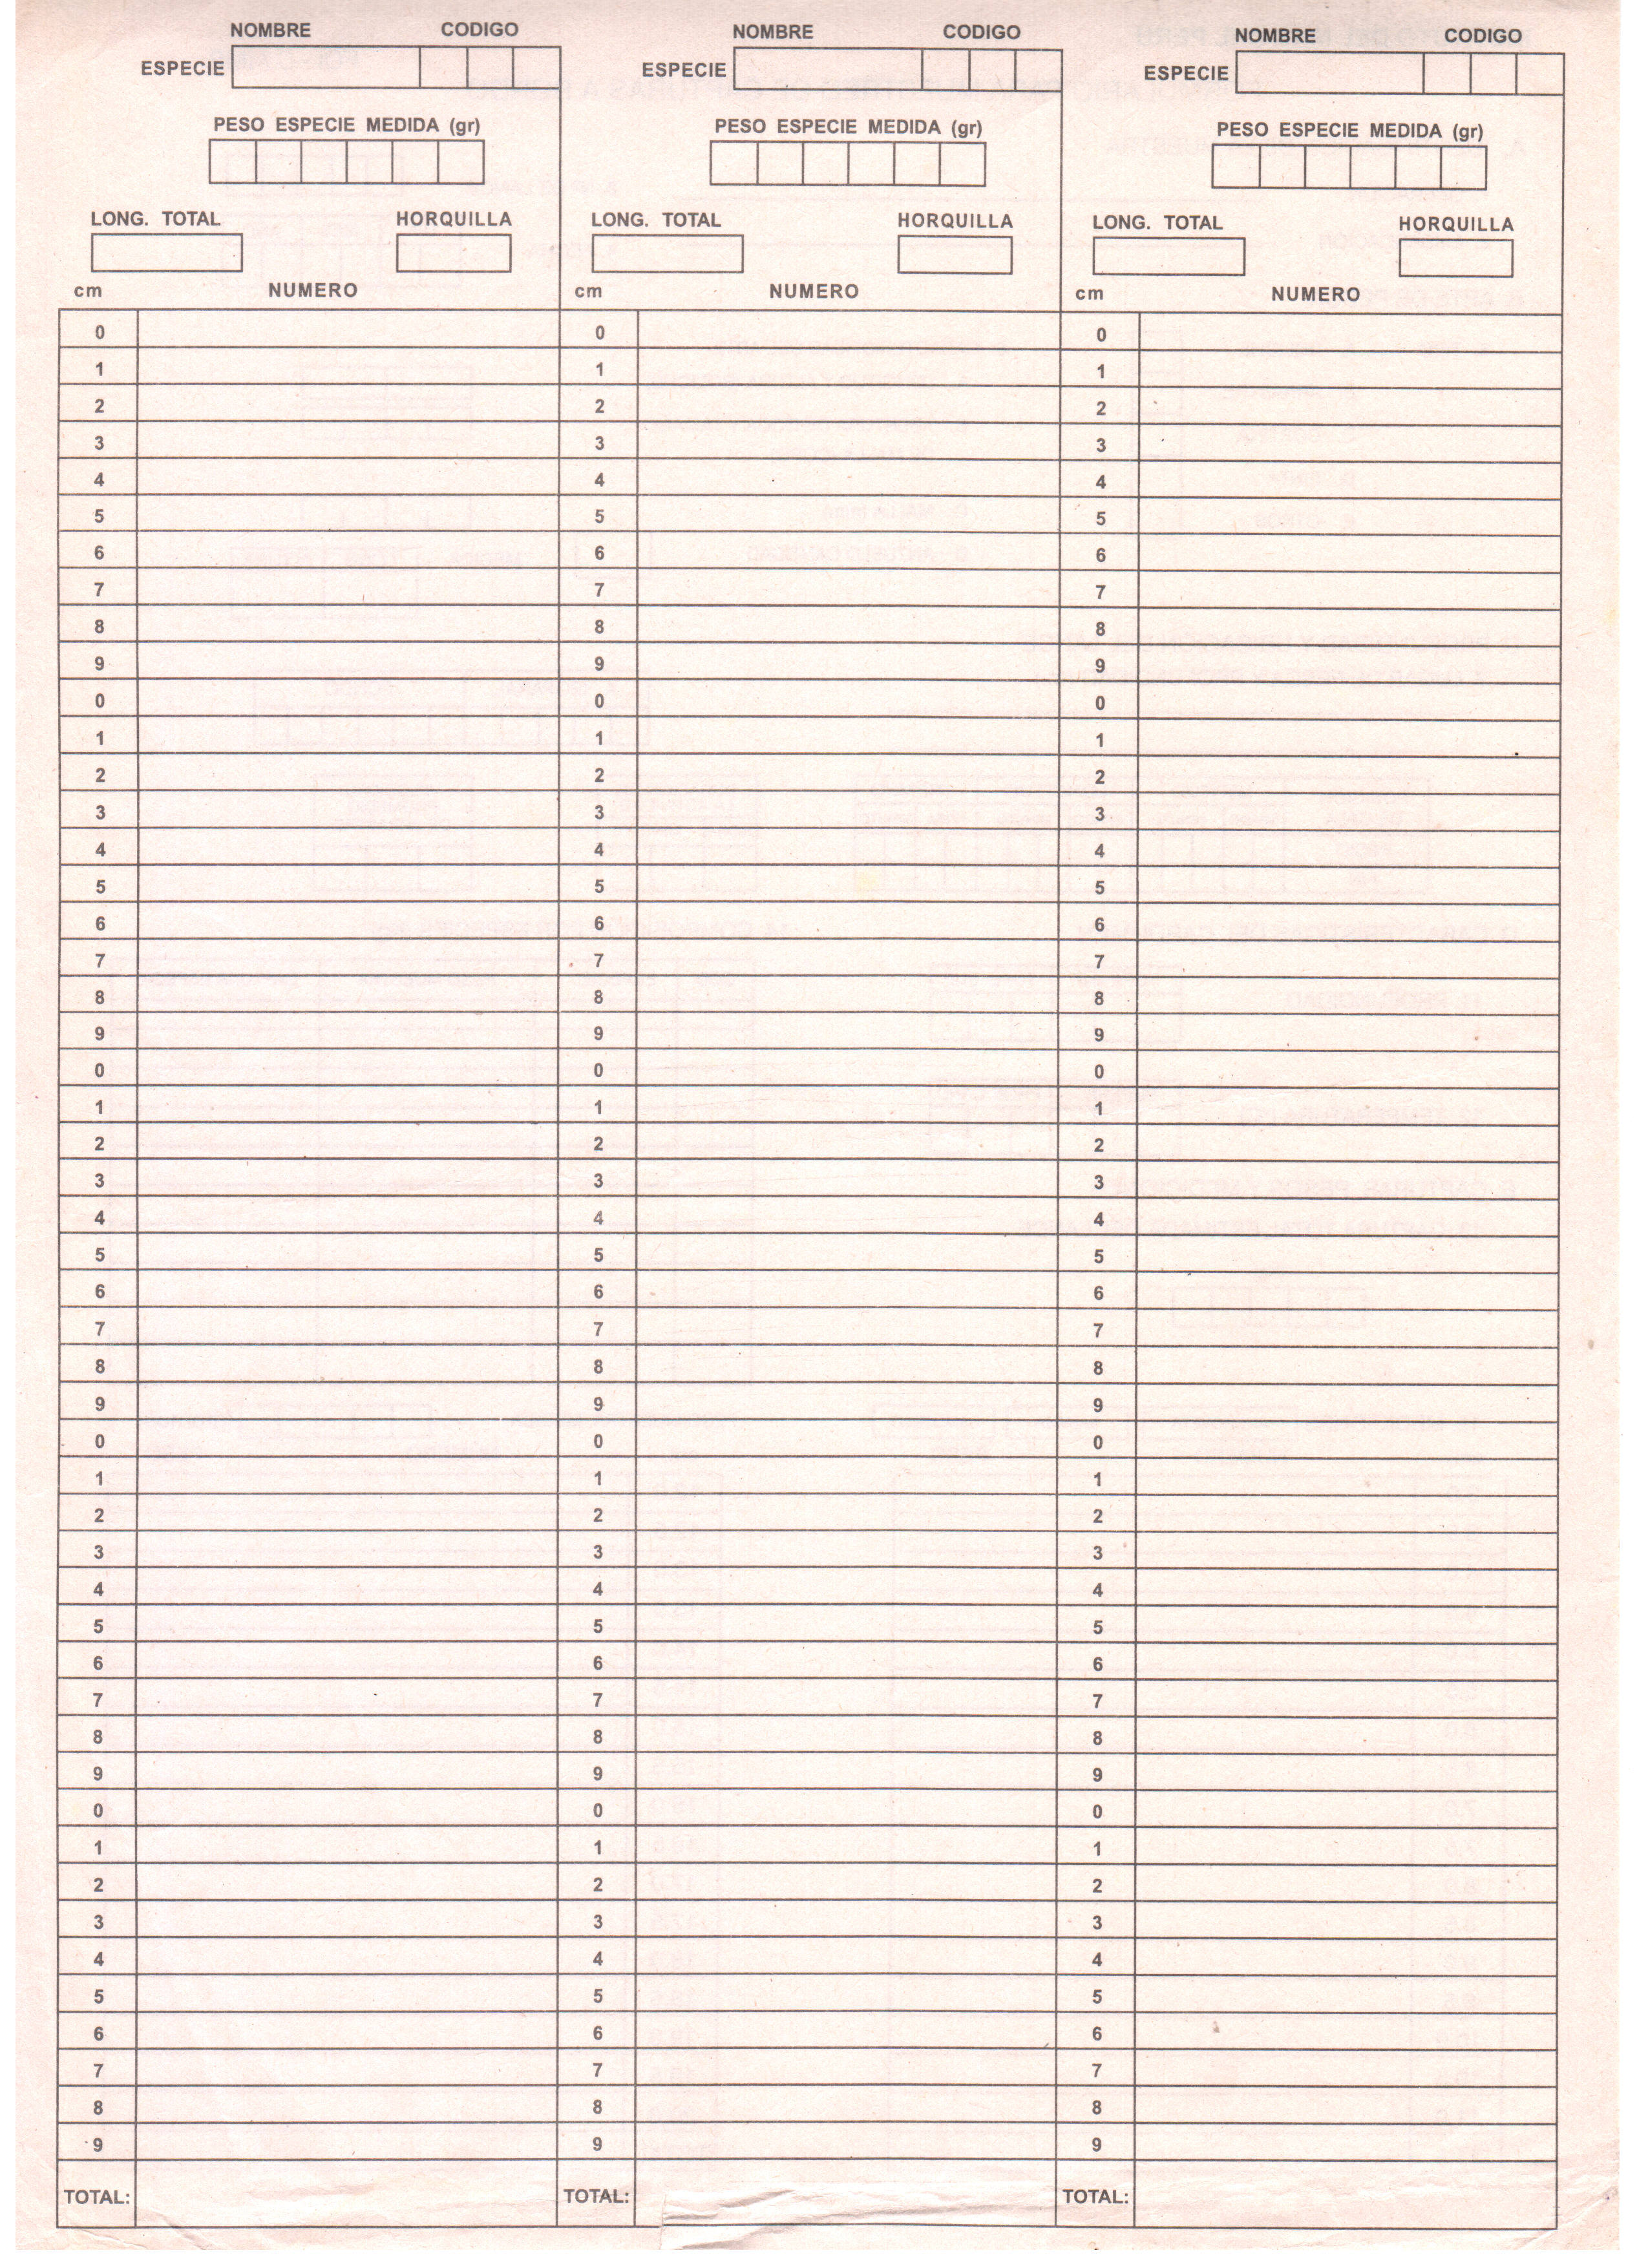
\includegraphics[scale=0.35]{imagen_manual_OPEMAR/ficha23.jpg}} %\caption{Ficha: Secci�n A: Indentificaci�n de la muestra}
    \end{center}
    \end{figure}
  
 % % % % %A�adir significado para cada uno
 
 
 
 
 
\chapter{¿Cómo ingresar una ficha de OPEMAR?}
 
 
\section {Verificación de instalación.}
\begin{enumerate}
\item\textbf{Conexión de red:} Es necesario verificar la conexión correcta y buena del internet durante todo el proceso de digitación.
\item \textbf{Instalación del módulo-OPEMAR:} Verificar la correcta instalación del módulo OPERMAR, si la computadora no tuviera instalado el módulo, avisar a informática, llamando al anexo 926-Informática con el Sr. Oré o Juan Carlos.
\item \textbf{Creación del usuario y contraseña:} El digitador deberá entregar sus datos en el área de informática.
\item\textbf{ Acceso al sistema:} Verificar si encuentra su nombre dentro del listado de usuarios y así mismo colocar la contraseña para probar el correcto acceso.
\end{enumerate}


\section{Búsqueda del crucero}

\begin{itemize}
\item Ejemplo: En esta oportunidad le tocó digitar el crucero denominado:  \\\textbf{ C}rucero\textbf{ B}iomasa \textbf{D}esovante de \textbf{A}nchoveta y \textbf{S}ardina- \textbf{CR.0008-09.}
\item Buscar el ícono de \textbf{OPEMAR} en el escritorio.

 \begin{figure}[!h]
 \begin{center} 
\fbox{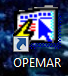
\includegraphics[scale=1.7]{imagen_manual_OPEMAR/OPEMAR.png}}
 \caption{Ícono del OPEMAR}
\end{center}
 \end{figure}

\item Una vez ingresado dirigirse a la casilla, ubicada en el extremo superior denominada \textbf{conexión}, aparecerá la casilla de búsqueda de usuarios, buscar su usuario y colocar su contraseña= D.N.I.


\begin{figure}[!h]
 \begin{center} 
\fbox{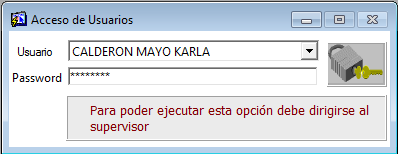
\includegraphics[scale=0.85]{imagen_manual_OPEMAR/usuario1.png}}
 \caption{Ícono del OPEMAR}
\end{center}
 \end{figure}

\item Primero ingresar por la sección tecnológica y colocar en la casilla búsqueda el código del crucero: 

\begin{center}
\fbox{\Large \textbf{0008-09}}
\end{center}

\begin{figure}[!h]
 \begin{center} 
\fbox{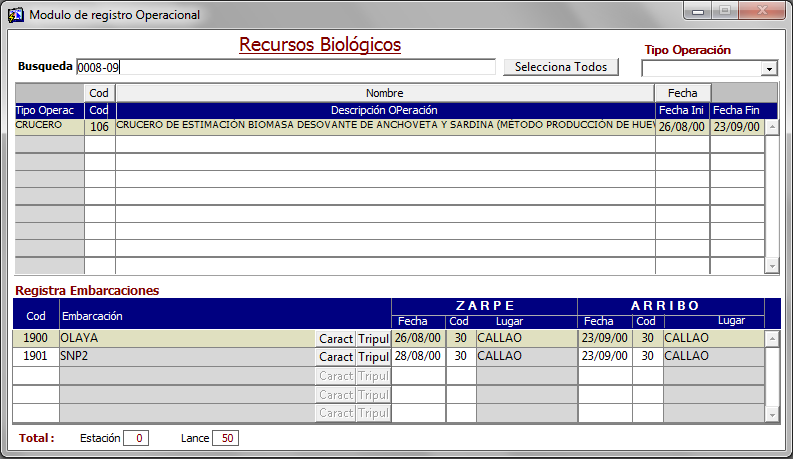
\includegraphics[scale=0.6]{imagen_manual_OPEMAR/busqueda.png}}
 \caption{Ícono del OPEMAR}
\end{center}
 \end{figure}

\newpage
\item Una vez ingresado el código, figurará en el encabezado el nombre del crucero, la embarcación, la fecha de inicio - final y el número de cala correspondiente.

\begin{figure}[!h]
 \begin{center} 
\fbox{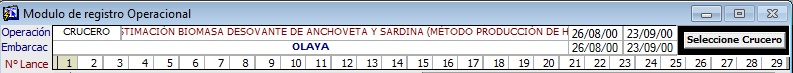
\includegraphics[scale=0.75]{imagen_manual_OPEMAR/encabezado.png}}
 \caption{Ícono del OPEMAR}
\end{center}
 \end{figure}

\item Dicha información figura en la ficha de la siguiente manera:
\item [] {\textbf{Operación:}} Cr. Biomasa Desovante 0008-09.
\item [] {\textbf{Embarcación:}} BIC José Olaya Balandra.



\begin{figure}[!h]
 \begin{center} 
\fbox{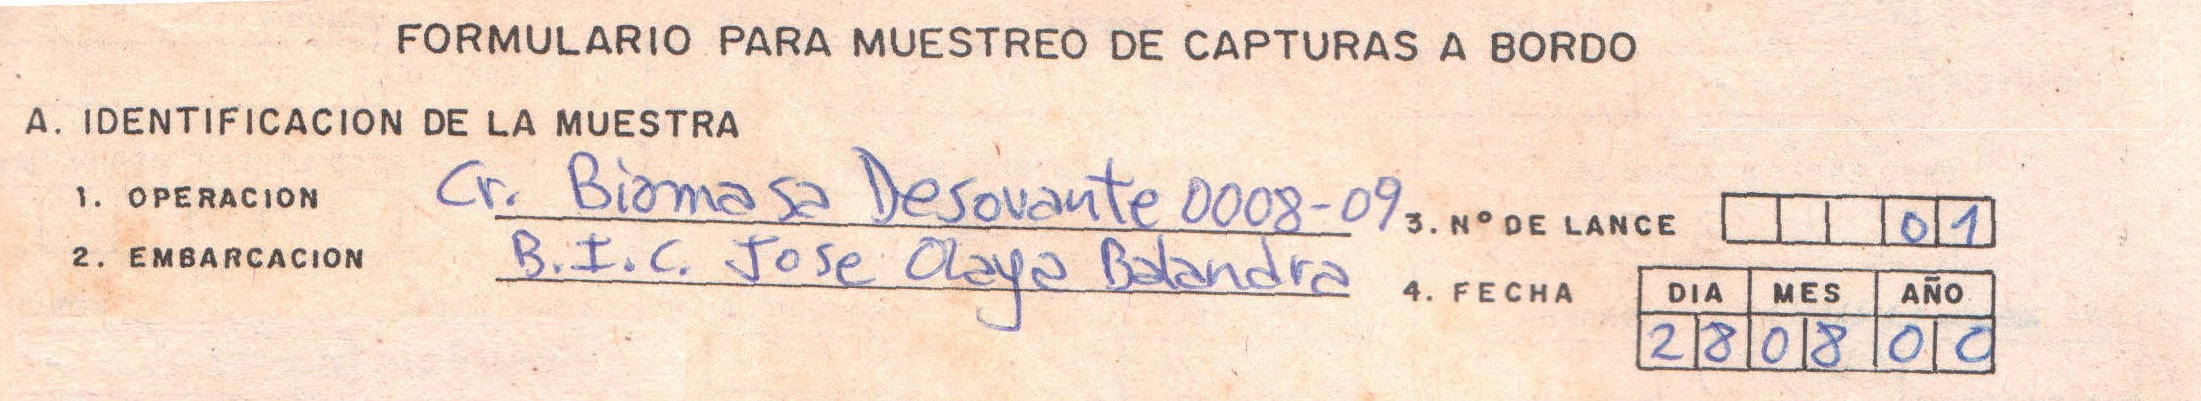
\includegraphics[scale=0.6]{imagen_manual_OPEMAR/casilla22.jpg}}
 \caption{Ícono del OPEMAR}
\end{center}
 \end{figure}




\newpage

\item Llenar la sección-bitácora. 


\begin{figure}[!h]
 \begin{center} 
\fbox{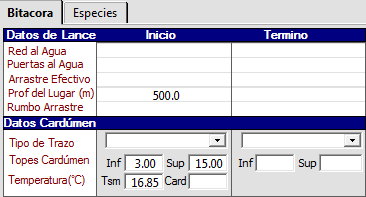
\includegraphics[scale=0.6]{imagen_manual_OPEMAR/bita1.png}}
 \caption{Ícono del OPEMAR}
\end{center}
 \end{figure}





\item Llenar la seccción-especies.
\item Salir de la casilla tecnológica, para luego añadir la información biológica.
\item Ficha biológica
\item Búsqueda del crucero, cala y especie.

\end{itemize}



\chapter{Casos presentados en la digitación de fichas-OPEMAR}

\chapter{Validación de cruceros}

\begin{itemize}
\item [ ] Para los procesos de validación de cruceros, se diseño un sistema que fuero capaz de registrar las fichas revisadas, el objetivo de insertar este sistema de revisado consiste en tener la seguridad de que las fichas fueron insertadas a un proceso de validación de datos, lo que involucra que los datos se encuentran correctamente digitados.
\item [] El sistema cuenta con los siguiente sectores de validación.

\end{itemize}

\section{Validación en sector: Tecnológico}

\begin{itemize}

\item Se recomienda primero realizar la validación de la sección: Tecnológico, ya que este sector es el encabezado y la base de esquema de cada crucero.

\begin{figure}[!h]
 \begin{center} 
\fbox{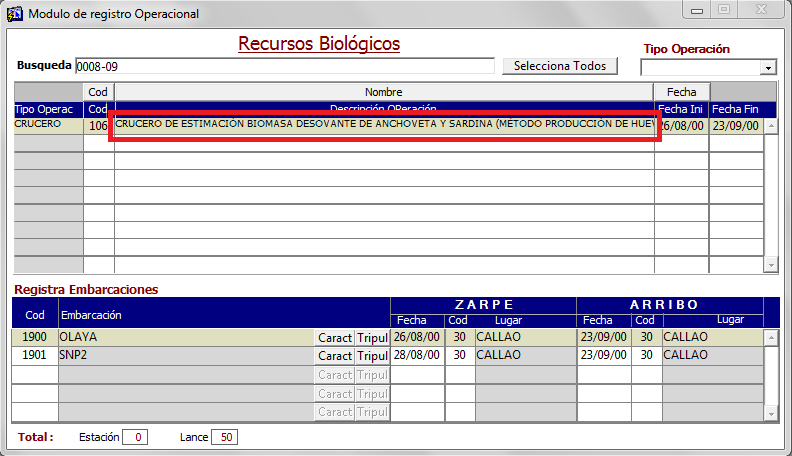
\includegraphics[scale=0.7]{imagen_manual_OPEMAR/sectorte.png}}
 \caption{Ícono del OPEMAR}
\end{center}
 \end{figure}

\item En este caso empezaremos con la embarcación: Olaya 


\begin{figure}[!h]
 \begin{center} 
\fbox{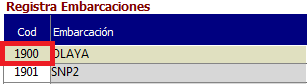
\includegraphics[scale=0.7]{imagen_manual_OPEMAR/casilla2.png}}
 \caption{Ícono del OPEMAR}
\end{center}
 \end{figure}


\item Seleccionada la opción, se ingresará al sector - tecnología.



\begin{figure}[!h]
 \begin{center} 
\fbox{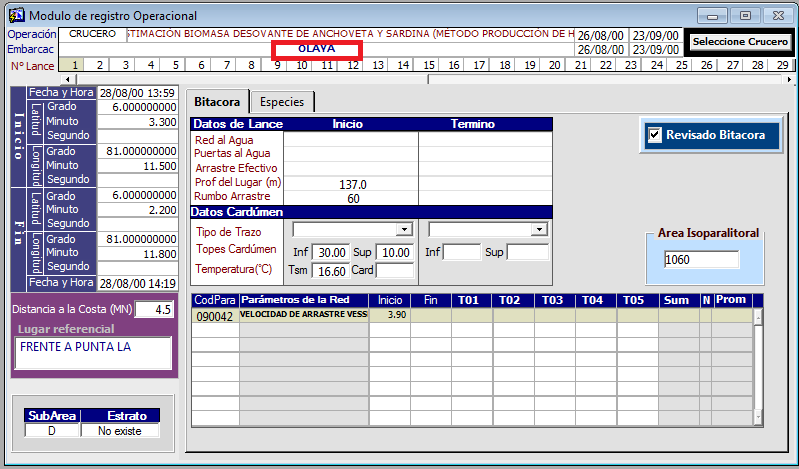
\includegraphics[scale=0.6]{imagen_manual_OPEMAR/olaya23.png}}
 \caption{Ícono del OPEMAR}
\end{center}
 \end{figure}

\item Al ingresar a la opción, deberá enfocarse en la revisión de:

\begin{enumerate}
\item \textbf{Coordenadas : }Verificar los grados y minutos 
\item \textbf{ Número Total de calas:} Sin repeticiones ni números intercalados
\item \textbf{Sección bitácora: }Incluye la verificación de datos del lance y del cardúmen.
\item \textbf{Área isoparalitoral:} Los cuatro números correctamente digitados.
\item \textbf{Velocidad de arrastre:} Verificar los datos.
\end{enumerate}

\newpage

\item Una vez verificada la correcta digitación de los datos, hacer click en la casilla: Revisado Bitácora.

\begin{figure}[!h]
 \begin{center} 
\fbox{
\includegraphics[scale=1]{imagen_manual_OPEMAR/revi23.png}}
 \caption{Ícono del OPEMAR}
\end{center}
 \end{figure}






\end{itemize}





\section{Validación en sector: Biológico}







\mainmatter  




\label{ch:capituloB} 
% ... (contenido del cap�tulo B)

\appendix % Ap�ndices 
\chapter{Apéndice X} 
\label{ch:apendiceX} 

% ... (contenido del ap�ndice X)

\chapter{Apéndice Y} 
\label{ch:apendiceY} 
% ... (contenido del ap�ndice Y)


\tableofcontents  Tabla de contenido 



\newpage 
\listoffigures  Índice de figuras 
\newpage 
\listoftables  Índice de tablas 
\newpage 



\backmatter 
% Bibliograf�a 
\include{bibliografia}


\end{document}